\documentclass[a4paper,10pt]{article}

\usepackage[utf8]{inputenc}
\usepackage{epsfig}
\usepackage{amsmath}
\usepackage{amssymb}
\usepackage{array}
\usepackage{float} 
\usepackage{ctable}
\usepackage{multirow}
\usepackage{graphicx}
\usepackage{caption}
\usepackage{subcaption}
\usepackage{amsfonts}
\usepackage{cite}
%\usepackage{algorithmic}
\usepackage[]{algorithm2e}

\usepackage{listings}
\lstset{breaklines=true} 


\def\th{^{th}}
\newcommand{\bs}[1]{\boldsymbol{#1}}
\newcommand{\pop}{\mathcal{P}}

\def\th{^{th}}
\def\pd{\frac{\partial}{\partial q_i^k}}
\newcommand{\mcf}[1]{p\Big( \norm{\bs{#1}^k}_1 \Big)}
\def\pdy{\frac{\partial}{\partial y_i^k}}
\def\pdq{\frac{\partial}{\partial q_i^k}}
\newcommand{\diag}{\mathop{\mathrm{diag}}}
%\newcommand{\bs}[1]{\boldsymbol{#1}}
\newcommand{\norm}[1]{\left\lVert#1\right\rVert}

\newcommand{\normb}[1]{\left\lVert \bs{#1} \right\rVert_1}


\usepackage{autonum}


\title{Population Dynamics Toolbox}
\author{Carlos Barreto}

\begin{document}

\maketitle



\begin{abstract}
 This is set of tools to implement evolutionary dynamics with multiple populations. We consider both small and large populations. For finite populations, we implement some revision protocols to model random interactions between agents. On the other hand, the evolution of a society with large populations is approximated by means of dynamical equations. 
 
 The toolbox is designed to facilitate the implementation of any game, as well as the implementation of different evolutionary dynamics and/or revision protocols.  In particular, our attempt is to make an efficient implementation of the algorithms to compute the dynamical evolution of the society. Also, the toolbox counts with some functions to plot the state of the system and the evolution of each strategy.
 
 
 
 
 
\end{abstract}


\tableofcontents



\section{Introduction}


% notation

Let us define a society of $\pop = \{ 1, \ldots, P\}$ composed by $P \geq 1$ populations. Each population consist of a large number of agents, which conform a mass $m^p > 0$, with $p \in \pop$. 
Let $S^p = \{ 1, \ldots, n^p \}$ be the set of actions (or pure strategies) available for each agent of the $p\th$ population. 
Each agent selects a pure strategy and the resulting state of the population is the usage proportion of each strategy. The set of population states is defined as $X^p = \{ x^p \in \mathbb{R}_+^{n^p} : \sum_{i \in S^p} x_i^p = m^p \}$, where the $i\th$ component of the state, denoted by $x_i^p \in \mathbb{R}_+$, is the mass of players that select the $i\th$ strategy of the population $p$.

Population games (or large games) capture some properties of the interactions of many economic agents:

\begin{enumerate}
\item large number of agents.
\item Continuity: The actions of an agent has small impact on the payoff of other agents.
\item Anonymity: means that the utility of each agent only depends on the aggregated actions of the other agents.
\end{enumerate}



In particular, an economic agent decides whether to modify or not its strategy according to the available information. In this respect, we assume that the agent's behavior satisfies both inertia and myopia properties. On the one hand, inertia 
is the tendency to remain at the status-quo, unless there exist motives to do that.
Also, this implies that the strategy adjustment events are rare events.
On the other hand, myopia means that the information used to make decisions is limited, e.g., each user makes decisions based on the current state of the population and do not estimate future actions. These two properties are based on the population games theoretical framework \cite{sandholm_book}
and behavioral economics \cite{gal}.

To accomplish the inertia property, the time between two successive updates of one 
agent's strategy is modeled with an exponential distribution (this distribution is used to model the occurrence of rare events). 
Thus, strategy actualization events could be characterized by means of stochastic alarm clocks.
Particularly, a rate $R_i$ Poisson alarm clock produces time among rings described by
a rate $R_i$ exponential distribution.
%These probabilities distributions are widely used by their memory-less property in stochastic analysis \cite{boyd, acemoglu2010, sandholm_book}. Thus, when all the agents of the population are provided with a rate $R_i$ Poisson alarm clock,
The whole actualization events in the population can be considered as a rate $R=\sum_{j\in \mathcal{V}} R_j$ Poisson alarm clock.
Therefore, the average number of events in a given time interval is $R$ and the probability of selecting the $i^{th}$
agent in a given time instant is
 $\frac{R_i}{R}$ \cite{sandholm_book}.

At each update opportunity (revision opportunity), the $i\th$ agent might compare the average profit of its strategy with the average profit of other strategies. Particularly, an agent might change its strategy with rate $\rho_{ij}$.
 
 The rate of change $\rho_{ij}$ is determined by a revision protocol, which defines the procedure used by each user to decide whether to change or not its strategy. The scalar $\rho_{ij} (\pi^p, x^p)$ is the \emph{conditional switch rate} from strategy $i$ to strategy $j$ in function of a given payoff vector $\pi$ and a population state $x^p$.
 
 Using the law of large numbers we can approximate the evolution of the society's state to a dynamical equation defined by
 \begin{equation}\label{eq:mean_dynamic}
  \dot{x}_i^p = \sum_{j\in S^p} x_j^p \rho_{ij} (\pi^p, x^p) - x_i^p \sum_{j\in S^p} \rho(\pi^p, x^p).
 \end{equation}
The previous equation is known as the \emph{mean dynamic}, which is used to define  some of the dynamics in the next section.

 
 
 \section{Revision Protocols and Evolutionary Dynamics}\label{sec:protocols}
 
 
In this section we introduce four revision protocols, that lead to the evolutionary dynamics \emph{logit dynamics} (Logit), \emph{replicator dynamics} (RD), \emph{Brown-von Neumann-Nash dynamics} (BNN), and \emph{Smith dynamics} (Smith). These dynamics belong to the families of \emph{perturbed optimization}, \emph{imitative dynamics}, \emph{excess payoff dynamics}, and \emph{pairwise comparison dynamics}, respectively \cite{hofbauer2001nash, sandholm_book}. 
 
 
 
 
 \subsection{Pairwise Proportional Imitation (Replicator Dynamics)}

The $i\th$ agent observes an opponent $j$ at random. Then it might change its strategy if  its opponent has a greater fitness. The rate change is 
%
\begin{equation}
\rho_{ij}^p(\pi^p, x^p) = \frac{1}{m^p} [\pi_j^p - \pi_i^p]_+
\end{equation}
%In this case, $x_j$ need not be observed. 
This protocol lead to the replicator dynamics defined as
\begin{equation}\label{eq:replicator}
\dot{x}_i^p = x_i^p \, \hat{F}_i^p \left( x \right),
\end{equation}
where $\hat{F}_i^p$ is the excess payoff to strategy $i\in S^p$, which is defined as   
\begin{equation}
\hat{F}_i^p (x) =  F_i^p(x) - \bar{F}^p(x),
\end{equation}
and $\bar{F}^p(x)$ is the average payoff the population $p$, i.e., 
\begin{equation}
 \bar{F}^p(x) = \frac{1}{m^p} \sum_{j \in S^p} x_j^p F_j^p(x).
\end{equation}



\subsection{Comparison to the Average Payoff (Brown-von Neumann-Nash Dynamics (BNN))}

The $i\th$ agent selects a strategy at random and might switch to it if that strategy has a payoff above the average. The agent switch strategy with probability proportional to the excess payoff
%
\begin{equation}
\rho_{ij}^p(\pi^p, x^p) = \left[ \pi_j^p - \frac{1}{m^p} \sum_{k\in S^p} x_k^p \pi_k^p \right]_+
\end{equation}

This protocol lead to BNN dynamics, defined as 
\begin{equation}\label{eq:bnn}
 \dot{x}_i^p = \left[ \hat{F}_i^p \left( \bs{x} \right) \right]_+ - x_i^p  \sum_{j \in S^p} \left[ \hat{F}_j^p \left( \bs{x} \right) \right]_+.
\end{equation}

\subsection{Pairwise Comparison (Smith Dynamics)}

The $i\th$ agent selects a strategy at random. If the opponent has a higher fitness, the the agent switch strategy with probability proportional to
\begin{equation}
\rho_{ij}(\pi, x) = \left[ \pi_j - \pi_i \right]_+
\end{equation}

This protocol leads to Smith dynamics that are defined as 
%
\begin{multline} 
\dot{x}_i^p  = \sum_{\gamma \in S^p} x_\gamma^p  \left[ F_i^p \left( \bs{x} \right) - F_\gamma^p \left( \bs{x} \right) \right]_+ 
%%\\
- x_i^p  \sum_{\gamma \in S^p} \left[ F_\gamma^p ( \bs{x}) - F_i^p( \bs{x} ) \right]_+.
\label{eq:smith}
\end{multline}



\subsection{Logit Choice}

The $i\th$ agent selects a strategy at random and change its strategy with a probability proportional to 

\begin{equation}
\rho_{ij}(\pi) = \frac{ \exp(\pi_j \eta^{-1} ) }{ \sum_{k \in S} \exp(\pi_k \eta^{-1} ) }
\end{equation}

This protocol belong to target dynamics and with a large population results in the following dynamics
\begin{equation}\label{eq:logit}
 \dot{x}_i^p = \frac{ \exp\left(\eta^{-1} F_i^p (\bs{x}) \right) }{ \sum_{\gamma \in S^p} \exp\left(\eta^{-1} F_\gamma^p (\bs{x}) \right) }, \, \, \eta>0,
\end{equation}
known ad Logit dynamics. 




\iffalse
\subsection{Maynard Smith Replicator}

\begin{equation}
\dot{x}_i = \frac{ x_i F_i }{ \bar{F}(x) } - x_i
\end{equation}
\fi




\subsection{Examples}



\begin{figure}[th]
  \centering
  \begin{subfigure}[b]{0.4\textwidth}
	  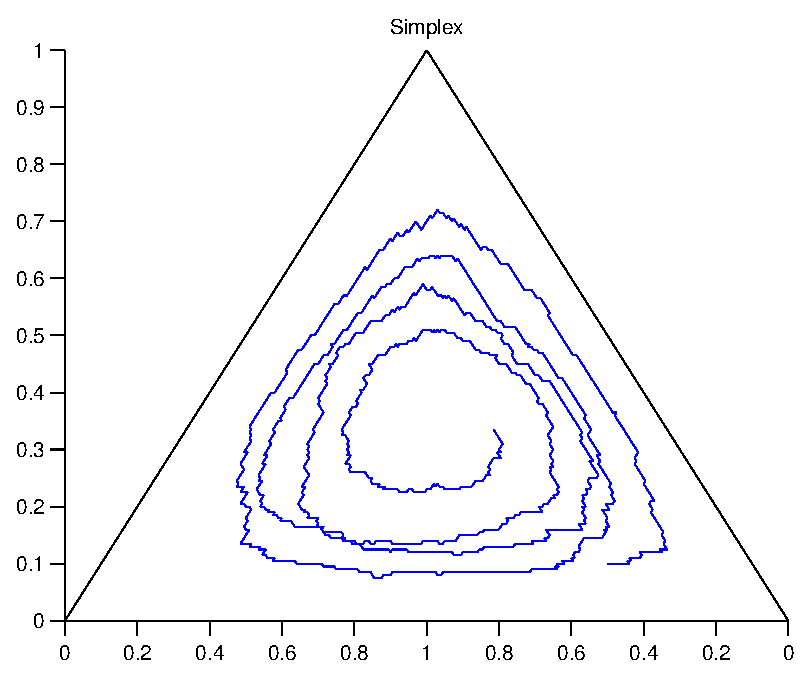
\includegraphics[width=\textwidth]{./images/test_finite_proportional_imitation.eps}
	  \caption{Small population.}
	  \label{fig:finite1_protocol}
  \end{subfigure}
  ~ 
  \begin{subfigure}[b]{0.4\textwidth}
	  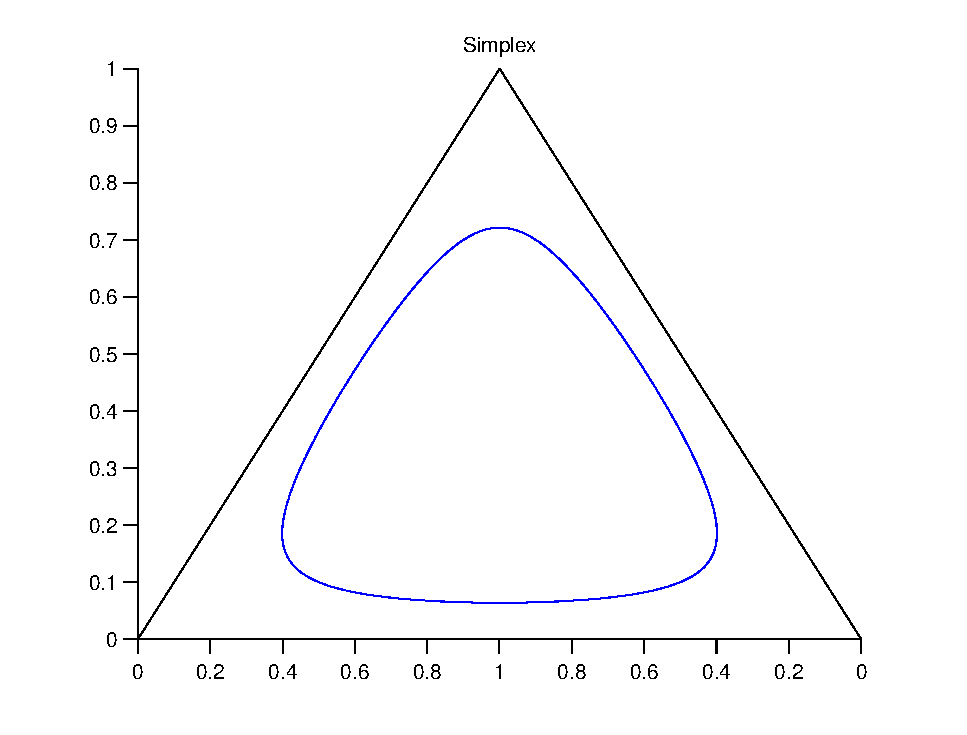
\includegraphics[width=\textwidth]{./images/test1_simplex_rd.eps}
	  \caption{Large popultion.}
	  \label{fig:finite1_dynamics}
  \end{subfigure}
  \caption{Rock-paper-scissors game with a) proportional imitation revision protocol and b) replicator dynamics.}
  \label{fig:finite1}
\end{figure}


\begin{figure}[th]
  \centering
  \begin{subfigure}[b]{0.4\textwidth}
	  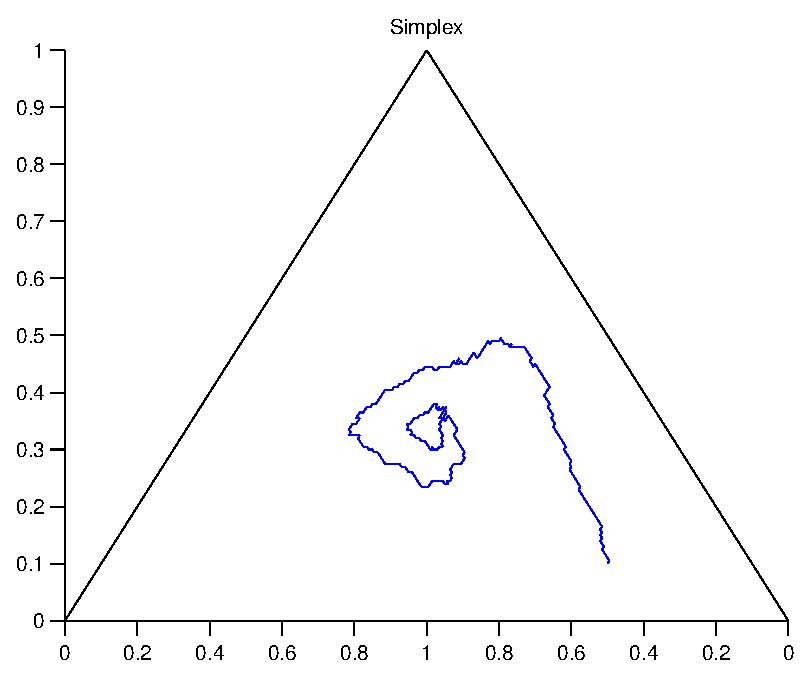
\includegraphics[width=\textwidth]{./images/test_finite_comparison2average.eps}
	  \caption{Small population.}
	  \label{fig:finite2_protocol}
  \end{subfigure}
  ~ 
  \begin{subfigure}[b]{0.4\textwidth}
	  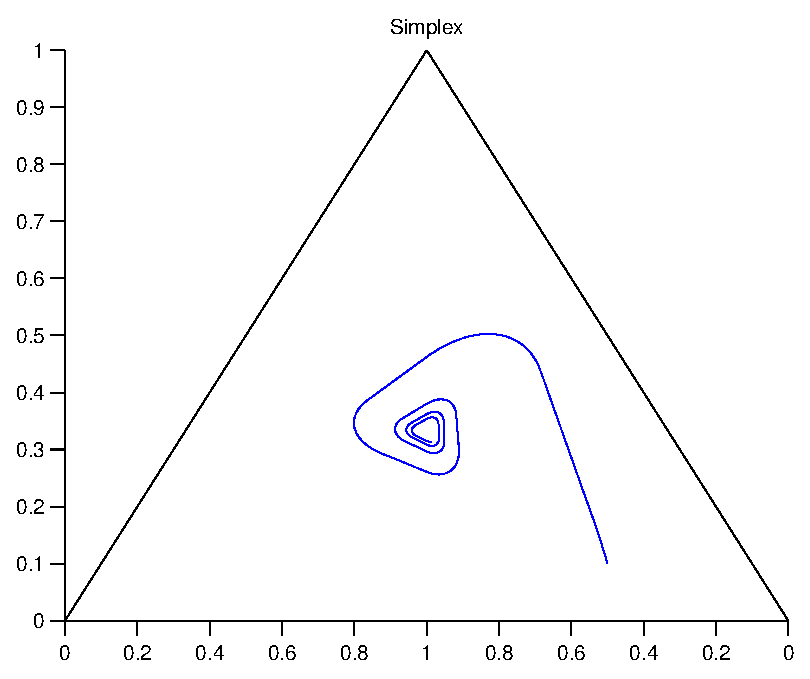
\includegraphics[width=\textwidth]{./images/test1_simplex_bnn.eps}
	  \caption{Large popultion.}
	  \label{fig:finite2_dynamics}
  \end{subfigure}
  \caption{Rock-paper-scissors game with a) comparison to average revision protocol and b) BNN dynamics.}
  \label{fig:finite2}
\end{figure}


\begin{figure}[tbh]
  \centering
  \begin{subfigure}[b]{0.4\textwidth}
	  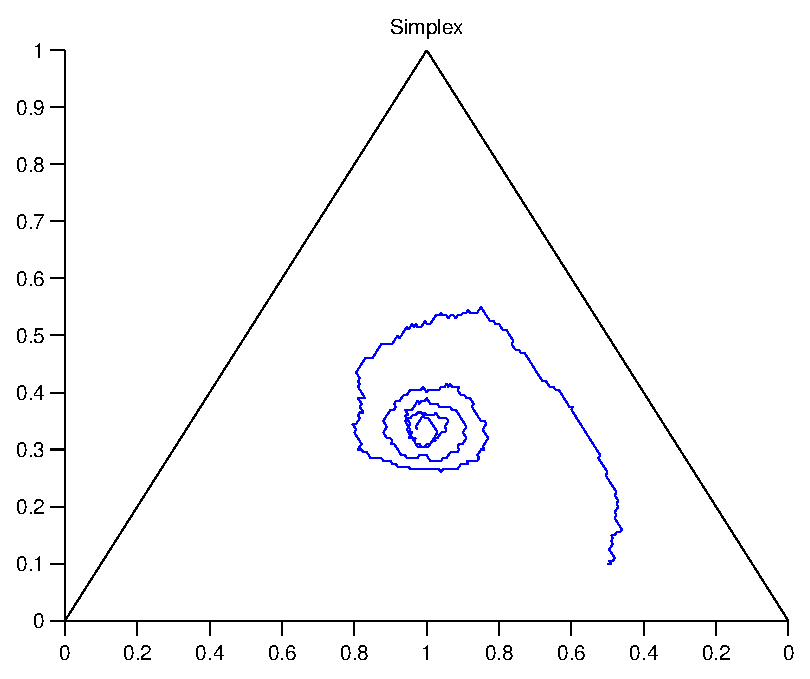
\includegraphics[width=\textwidth]{./images/test_finite_pairwise_comparison.eps}
	  \caption{Small population.}
	  \label{fig:finite3_protocol}
  \end{subfigure}
  ~ 
  \begin{subfigure}[b]{0.4\textwidth}
	  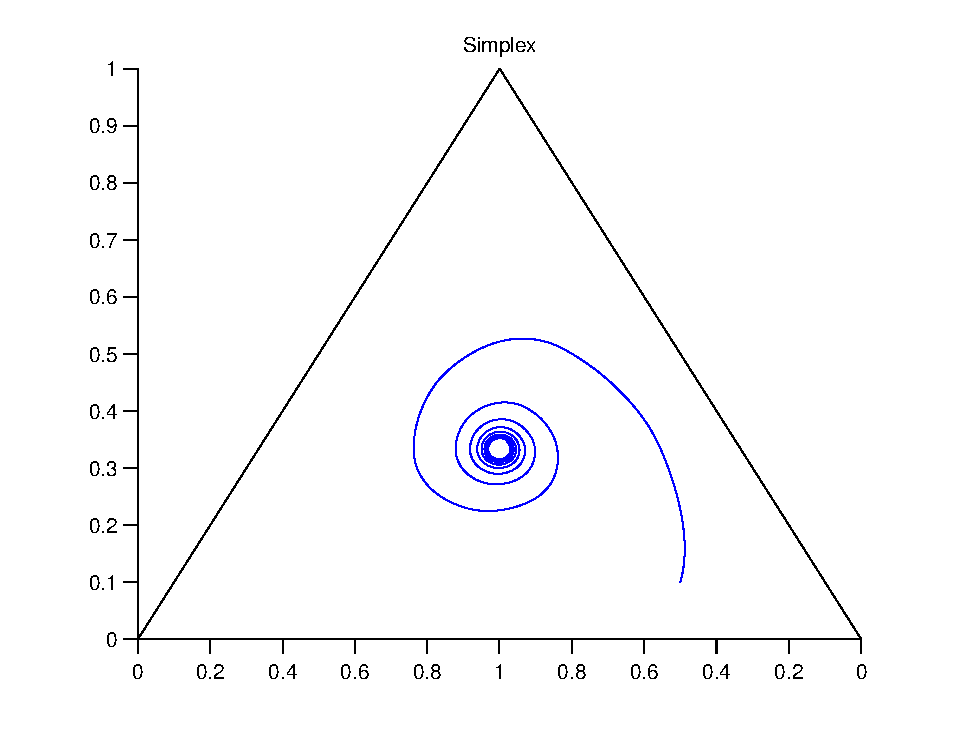
\includegraphics[width=\textwidth]{./images/test1_simplex_smith.eps}
	  \caption{Large popultion.}
	  \label{fig:finite3_dynamics}
  \end{subfigure}
  \caption{Rock-paper-scissors game with a) pairwise comparison revision protocol and b) Smith dynamics.}
  \label{fig:finite3}
\end{figure}


\begin{figure}[tbh]
  \centering
  \begin{subfigure}[b]{0.4\textwidth}
	  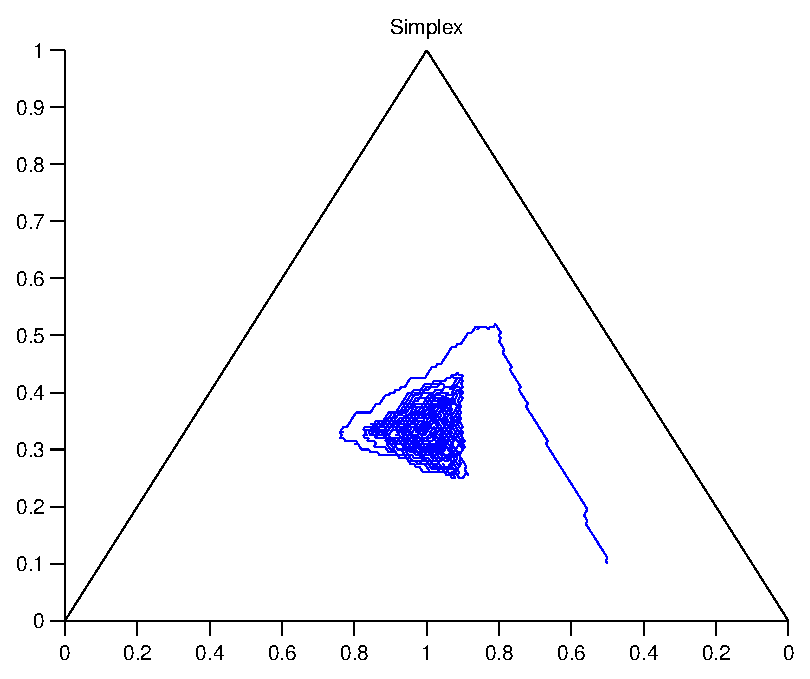
\includegraphics[width=\textwidth]{./images/test_finite_logit_choice.eps}
	  \caption{Small population.}
	  \label{fig:finite4_protocol}
  \end{subfigure}
  ~ 
  \begin{subfigure}[b]{0.4\textwidth}
	  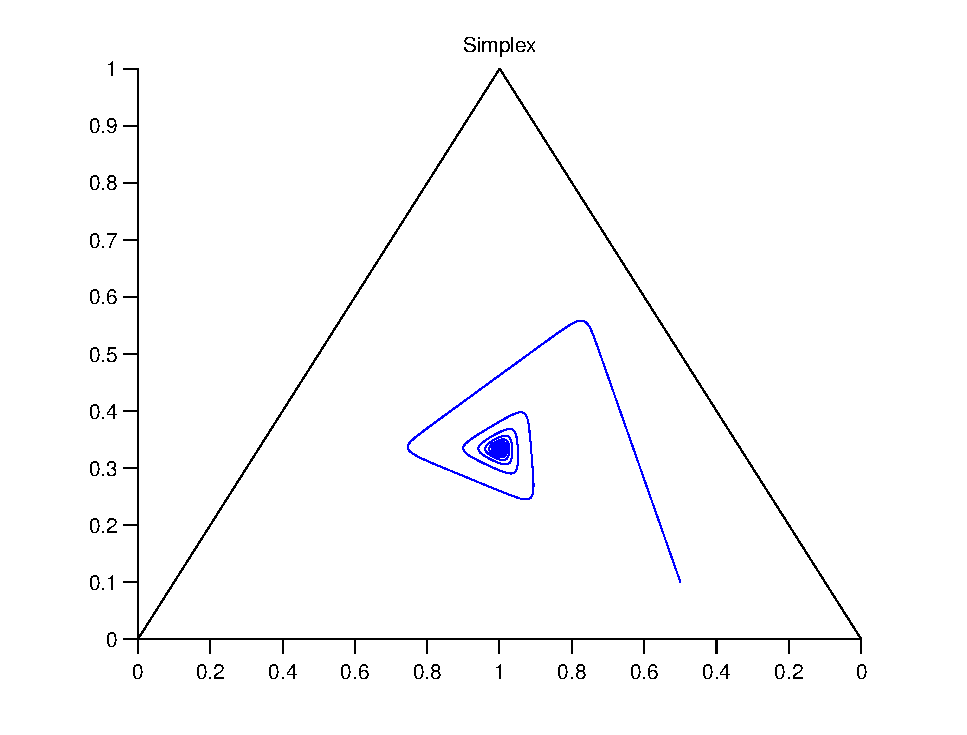
\includegraphics[width=\textwidth]{./images/test1_simplex_logit.eps}
	  \caption{Large popultion.}
	  \label{fig:finite4_dynamics}
  \end{subfigure}
  \caption{Rock-paper-scissors game with a) logit choice revision protocol and b) Logit dynamics with $\eta=0.02$.}
  \label{fig:finite4}
\end{figure}





In this section, we implement rock-paper-scissors game with both revision protocols and evolutionary dynamics presented above, to observe the behavioral differences between a society with small number of agents and its approximation to a dynamical system.
The game has only one population with three strategies, denoted $x = [x_1, \, x_2, \, x_3]^\top$. The fitness function is defined as $F(x)=Ax$, where A is equal to 
\begin{equation}
  A = \begin{pmatrix}
  2  & 1 &  3 \\
  3  & 2 &  1 \\
  1 &  3 &  2
  \end{pmatrix}
\end{equation}
Note that we modify the payoff matrix proposed in the literature to ensure positive payoffs.
Fig. \ref{fig:finite1} to \ref{fig:finite4} show the evolution of the society with each revision protocol and its approximation to differential equations. We set the initial condition $x_0 = [0.2, \, 0.7, \, 0.1 ]^\top$. The small population cases are made with $200$ agents and $10000$ iterations. The dynamical cases are run during 
30 time units.


%The evolution might take place in days, months, years.

\section{Implementation} \label{sec:implementation}

\subsection{Parameters of the Implementation}


\begin{table}[tbh]
\begin{center}
\begin{tabular}{l | p{.55 \textwidth} | l}\hline
Field & Description & Default value\\ \hline
P & Number of populations & 1 \\
n & Number of pure strategies per population & - \\
S & Vector of pure strategies in each population & ones(G.P, 1) * G.n \\
m & Vector with the mass of each population & ones(G.P, 1) \\
x0 & Initial state of the society & random \\
f & Function that returns a vector with the fitness of each strategy of a population & - \\
ode & ODE solver for the evolutionary dynamics & `ode45' \\
dynamics & Evolutionary dynamic. Current version support combinations of {`rd', `maynard\_rd',  `bnn', `smith',  `logit'} & `rd' \\
gamma & Defines the weight given to each dynamic when using combined dynamics &  $\sum \gamma(i) = 1$ \\ \hline
\end{tabular}
\end{center}
\caption{Parameters of the dynamical implementation.}
\label{tab:req_a}
\end{table}




\begin{table}[tbh]
\begin{center}
\begin{tabular}{l| p{.5 \textwidth} |l}\hline
Field & Description & Default value \\ \hline
N & Number of agents & 100 \\
R & Rate of the Poisson clock & 1 \\
revision\_protocol & Revision protocol. The current version support one of the following: comparison2average, pairwise\_comparison, logit\_choice, proportional\_imitation. & 'proportional\_imitation' \\ \hline
\end{tabular}
\end{center}
\caption{Parameters of the revision protocol.}
\label{tab:req_b}
\end{table}




The toolbox uses a structure that contains all the parameters required to run the simulations. The parameters of a population game are defined in Table \ref{tab:req_a}. The following is an example to define a game with one population and three strategies per population:
%
\begin{lstlisting}
G = struct('n', 3, 'f', @fitness1, 'dynamics', {rd} ,  'ode', 'ode113', 'x0',  [0.2 .7 0.1 ]', 'time', 60);
\end{lstlisting}
%
$n$ defines the number of strategies per population, $f$ is a function handler that calculates the fitness of the strategies in each population, and $dynamics$ defines the name of the evolutionary dynamics that we want to use. The simulations are run using the ordinal differential equation (ODE) solver called $ode113$, with initial condition $x0 = [0.2, \, 0.7, \, 0.1 ]^\top$ during $60$ time units.
Note that the number of populations and the mass of each population are defined by default to one.  The simulation can be started by executing
%
\begin{lstlisting}
 G.run()
\end{lstlisting}




On the other hand, the following structure is used to define a population game with small number of agents per population:
%
\begin{lstlisting}
G = struct('N', 200, 'n', 3, 'f', @fitness1, 'x0',  [0.2 .7 0.1 ]', 'ode', 'ode113', 'time', 10000, 'eta', 0.02, 'revision_protocol', @proportional_imitation); 
\end{lstlisting}
%
The finite population case uses the same parameters than the dynamical implementation, except for the dynamical model. However, it is necessary to define the revision protocol  and the number of agents $N$ per population.
Table \ref{tab:req_b} contains the list of parameters required to run the revision protocol. The simulation of the revision protocol can be started by executing
\begin{lstlisting}
 G.run_finite()
\end{lstlisting}

The functions \verb|G.graph()| and \verb|G.graph_evolution()| can be used to graph the simplex and the state evolution of the society for both cases.



\subsection{Example: Rock-Paper-Scissors Game}



\begin{figure}[th]
  \centering
  \begin{subfigure}[b]{0.4\textwidth}
	  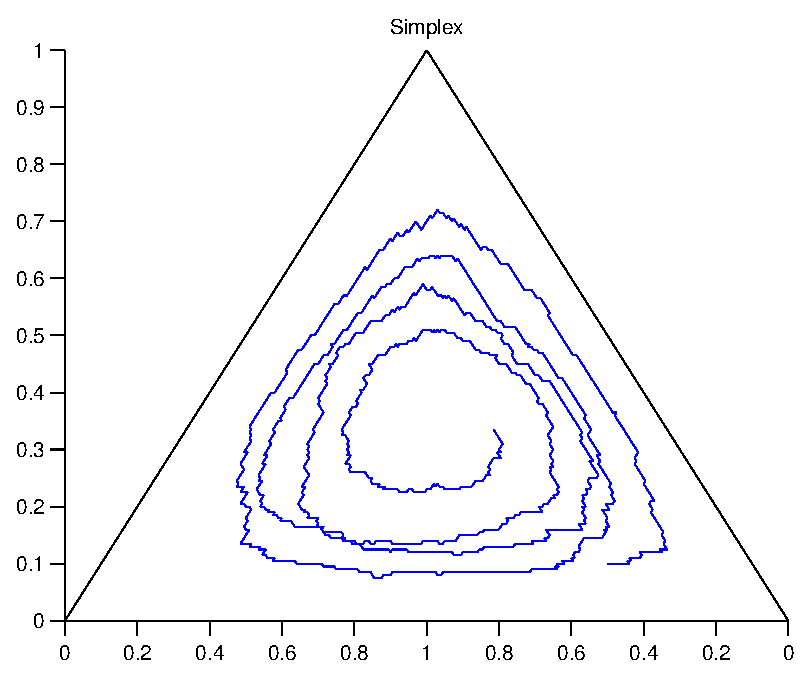
\includegraphics[width=\textwidth]{./images/test_finite_proportional_imitation.eps}
	  \caption{Small population.}
	  \label{fig:finite1_protocol}
  \end{subfigure}
  ~ 
  \begin{subfigure}[b]{0.4\textwidth}
	  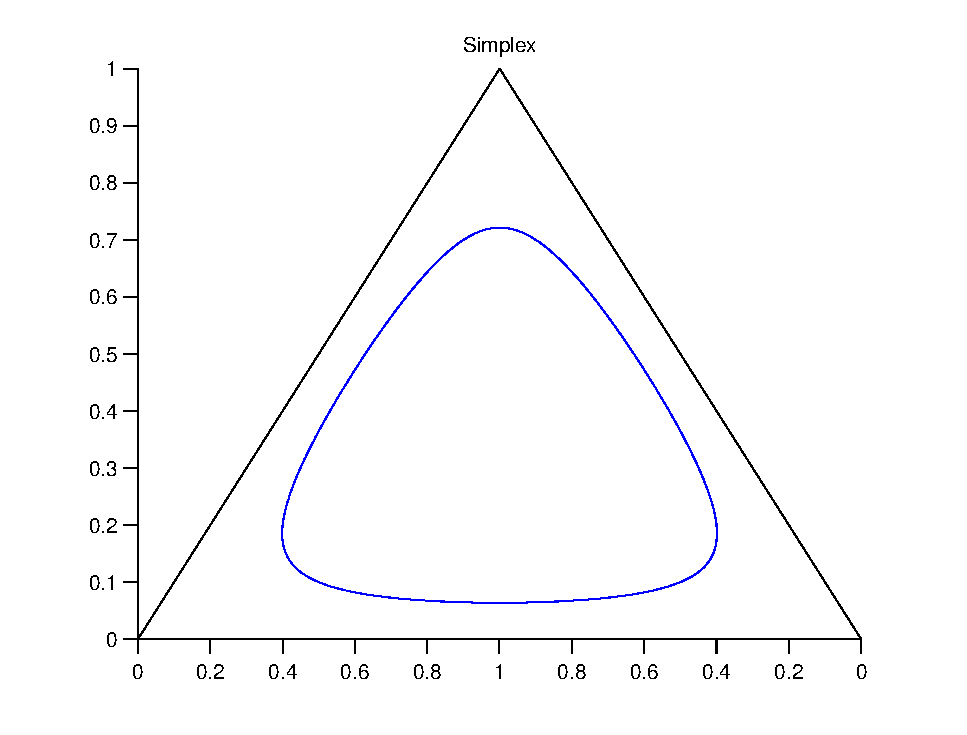
\includegraphics[width=\textwidth]{./images/test1_simplex_rd.eps}
	  \caption{Large popultion.}
	  \label{fig:finite1_dynamics}
  \end{subfigure}
  \caption{Rock-paper-scissors game with a) proportional imitation revision protocol and b) replicator dynamics.}
  \label{fig:finite1}
\end{figure}


\begin{figure}[th]
  \centering
  \begin{subfigure}[b]{0.4\textwidth}
	  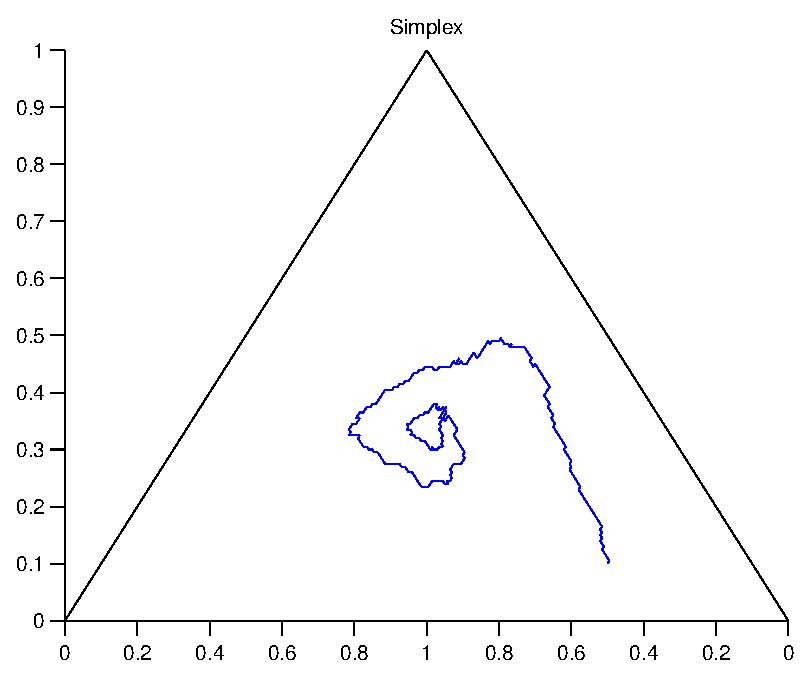
\includegraphics[width=\textwidth]{./images/test_finite_comparison2average.eps}
	  \caption{Small population.}
	  \label{fig:finite2_protocol}
  \end{subfigure}
  ~ 
  \begin{subfigure}[b]{0.4\textwidth}
	  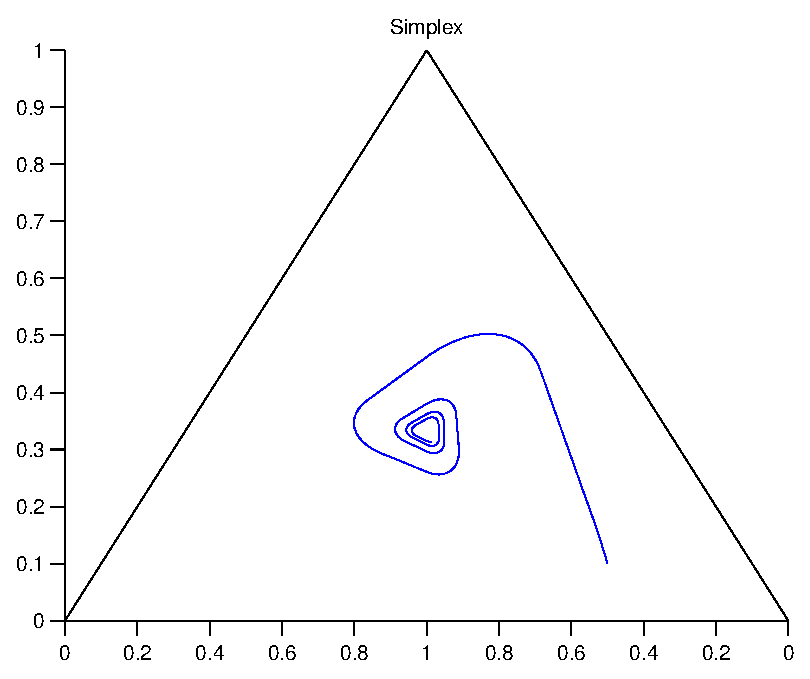
\includegraphics[width=\textwidth]{./images/test1_simplex_bnn.eps}
	  \caption{Large popultion.}
	  \label{fig:finite2_dynamics}
  \end{subfigure}
  \caption{Rock-paper-scissors game with a) comparison to average revision protocol and b) BNN dynamics.}
  \label{fig:finite2}
\end{figure}


\begin{figure}[tbh]
  \centering
  \begin{subfigure}[b]{0.4\textwidth}
	  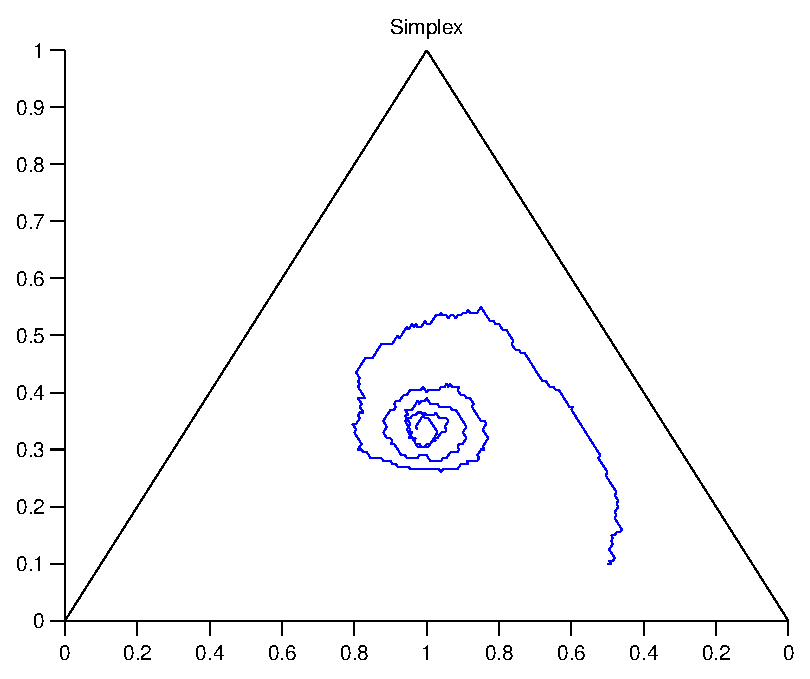
\includegraphics[width=\textwidth]{./images/test_finite_pairwise_comparison.eps}
	  \caption{Small population.}
	  \label{fig:finite3_protocol}
  \end{subfigure}
  ~ 
  \begin{subfigure}[b]{0.4\textwidth}
	  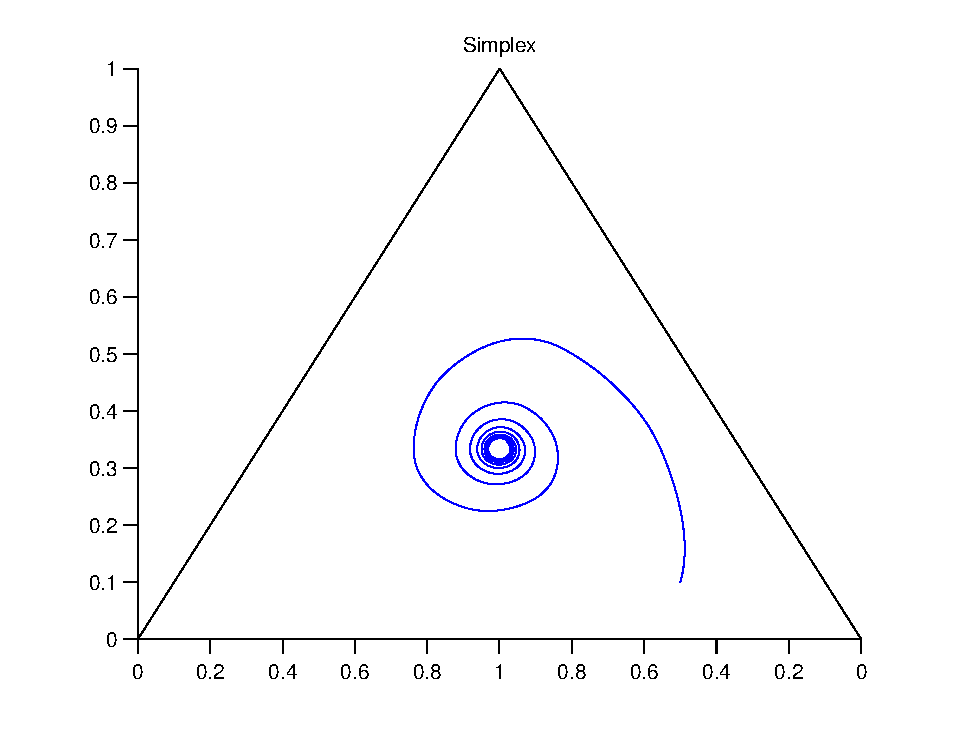
\includegraphics[width=\textwidth]{./images/test1_simplex_smith.eps}
	  \caption{Large popultion.}
	  \label{fig:finite3_dynamics}
  \end{subfigure}
  \caption{Rock-paper-scissors game with a) pairwise comparison revision protocol and b) Smith dynamics.}
  \label{fig:finite3}
\end{figure}


\begin{figure}[tbh]
  \centering
  \begin{subfigure}[b]{0.4\textwidth}
	  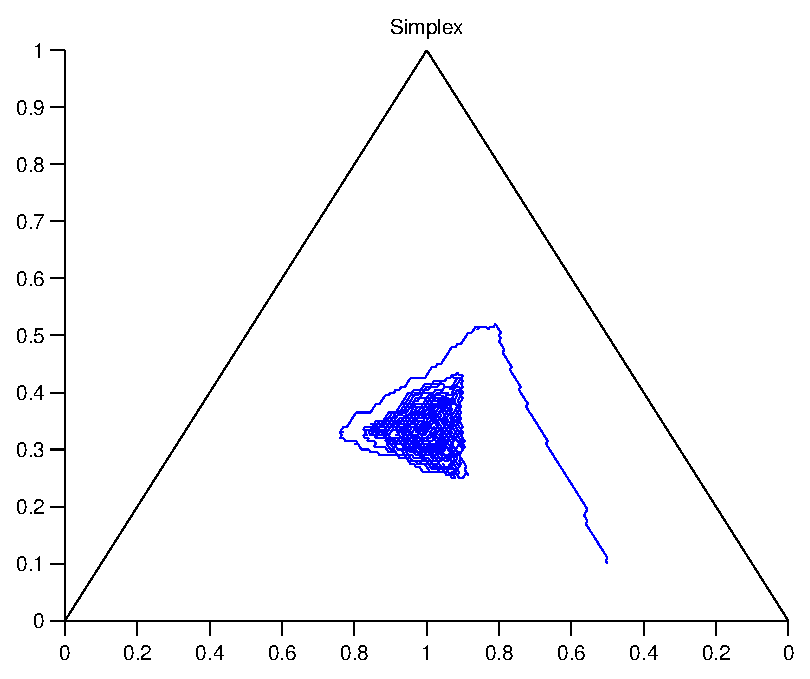
\includegraphics[width=\textwidth]{./images/test_finite_logit_choice.eps}
	  \caption{Small population.}
	  \label{fig:finite4_protocol}
  \end{subfigure}
  ~ 
  \begin{subfigure}[b]{0.4\textwidth}
	  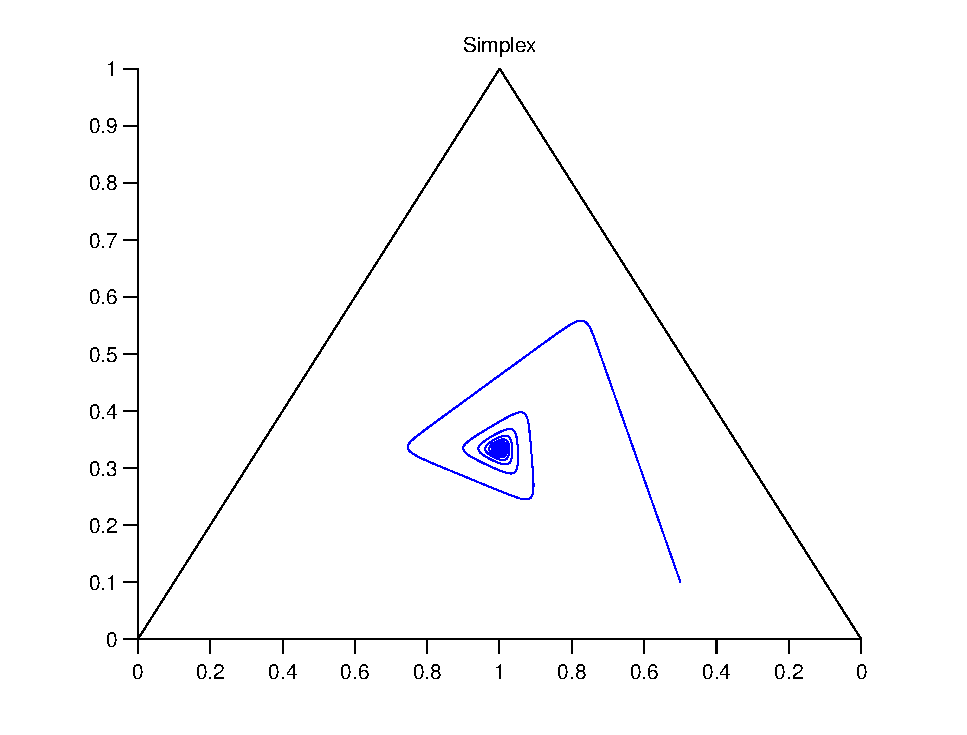
\includegraphics[width=\textwidth]{./images/test1_simplex_logit.eps}
	  \caption{Large popultion.}
	  \label{fig:finite4_dynamics}
  \end{subfigure}
  \caption{Rock-paper-scissors game with a) logit choice revision protocol and b) Logit dynamics with $\eta=0.02$.}
  \label{fig:finite4}
\end{figure}





In this section, we implement rock-paper-scissors game with both revision protocols and evolutionary dynamics presented above, to observe the behavioral differences between a society with small number of agents and its approximation to a dynamical system.
The game has only one population with three strategies, denoted $x = [x_1, \, x_2, \, x_3]^\top$. The fitness function is defined as $F(x)=Ax$, where A is equal to 
\begin{equation}
  A = \begin{pmatrix}
  2  & 1 &  3 \\
  3  & 2 &  1 \\
  1 &  3 &  2
  \end{pmatrix}
\end{equation}
Note that we modify the payoff matrix proposed in the literature to ensure positive payoffs.
Fig. \ref{fig:finite1} to \ref{fig:finite4} show the evolution of the society with each revision protocol and its approximation to differential equations. We set the initial condition $x_0 = [0.2, \, 0.7, \, 0.1 ]^\top$. The small population cases are made with $200$ agents and $10000$ iterations. The dynamical cases are run during 
30 time units.


%The evolution might take place in days, months, years.
















\section{Combined Dynamics}

It is possible to define a set of dynamics to run a combination of the dynamics. 
The resulting dynamic is defined as 
\begin{equation}
\dot{ x } = \sum_{d\in \mathcal{D}} \gamma_d V_d( x ),
\end{equation}
where $\mathcal{D}=\{ Logit, RD, Smith, BNN \}$ denotes the set of available dynamics, $V_d()$ is the differential equation of the $d\th$ dynamic and $\gamma_d$ is the weight assigned to it.
The dynamics should be defined in a cell array, e.g., 
\begin{lstlisting}
dynamics = {'bnn', 'rd'};
\end{lstlisting}
The combination is made making a linear combination between each dynamic listed in the cell array. The weight assigned to each dynamic is defined in the vector \verb|gamma|. In this case we assign 
\begin{lstlisting}
gamma = [.25, .75]; 
\end{lstlisting}

Fig. \ref{fig:rps_combined} shows an example of the combined dynamics for the rock-paper-scissors game. Note that the evolution of the system is not confined to a limit cycle, as happened with the replicator dynamics in Fig.  \ref{fig:finite1}.

\begin{figure}[h]
  \centering
  \begin{subfigure}[b]{0.4\textwidth}
	  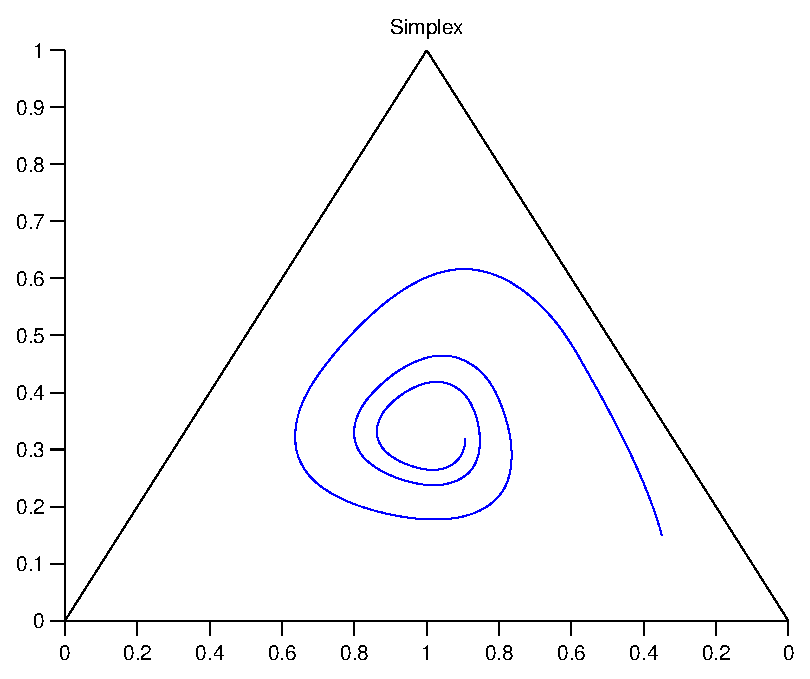
\includegraphics[width=\textwidth]{./images/test_combined.eps}
	  \caption{Simplex.}
	  \label{fig:test_combined_simplex}
  \end{subfigure}
  ~ 
  \begin{subfigure}[b]{0.45\textwidth}
	  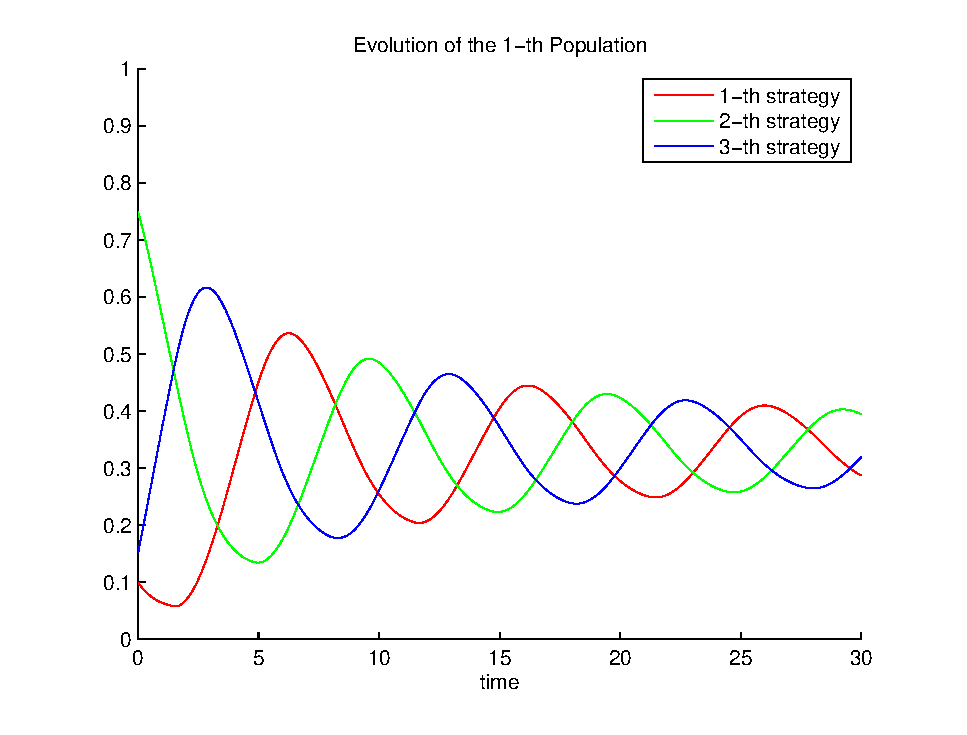
\includegraphics[width=\textwidth]{./images/test_combined_ev.eps}
	  \caption{Evolution of the strategies in time.}
	  \label{fig:test_combined_ev}
  \end{subfigure}
  \caption{Evolution of the combination of replicator dynamics and BNN dynamics.}
  \label{fig:rps_combined}
\end{figure}









%\newpage

\section{Multi-population Games}



%\subsection{Examples}

\subsection{Matching pennies}

We implement a matching pennies game defining a society $\pop = \{p_1, p_2\}$ with two populations and two strategies per population, namely \emph{heads} and \emph{tails}. First, note that the payoff of the game in normal form is
%
\begin{table}[H]
\centering
 \begin{tabular}{|c|c|} \hline
  2, 1 & 1, 2 \\ \hline
  1, 2 & 2, 1 \\ \hline
 \end{tabular}
\end{table}
%
%In this case, the state of populations $1$ and $2$ are denoted by x^1 and x^2, respectively. .
Now, the fitness vector of the  population $p_j$ can be expressed as $F^{p_j}(x^{p_k}) = A^{p_j} x^{p_k}$, for $p_j, p_k \in \pop$ and $p_j \neq p_k$. That is, the payoff of a population is affected only by the state of the opponent population.
%$x^p \in $  $p=\{x_h^p, x_t^p\}$. 
The payoff matrices are defines as follows
%
\begin{equation}
  A^1 = \begin{pmatrix}
2 & 1 \\
1 & 2 
  \end{pmatrix}
\end{equation}
%
\begin{equation}
  A^2 = \begin{pmatrix}
  1 & 2 \\
  2 & 1 
  \end{pmatrix}
\end{equation}
%
Fig. \ref{fig:mp_game_rd} to \ref{fig:mp_game_logit} show the evolution of the social state with the evolutionary dynamics presented in Section \ref{sec:protocols}. 

\begin{figure}[h]
  \centering
  \begin{subfigure}[b]{0.45\textwidth}
	  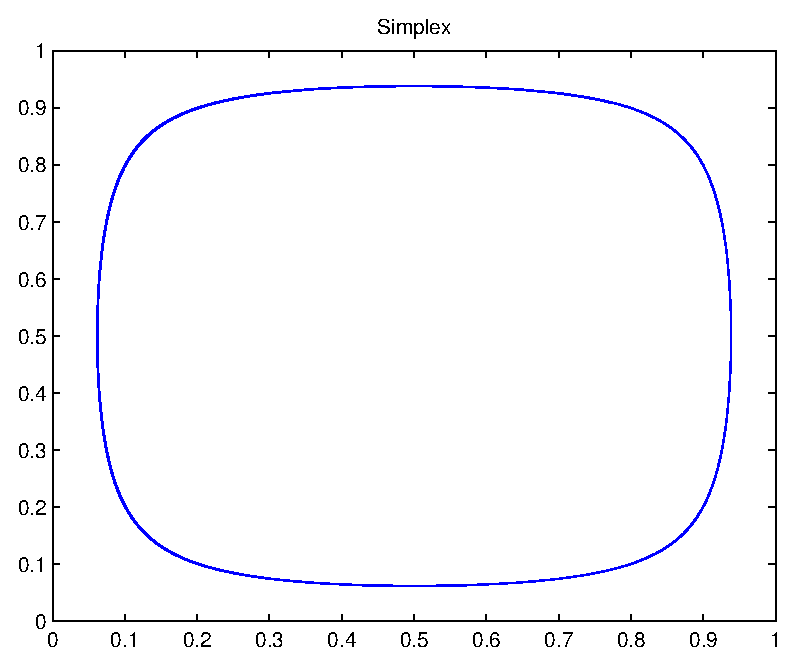
\includegraphics[width=\textwidth]{./images/test2_simplex_rd.eps}
	  \caption{Simplex.}
	  \label{fig:test2_simplex_rd}
  \end{subfigure}
  ~ 
  \begin{subfigure}[b]{0.45\textwidth}
	  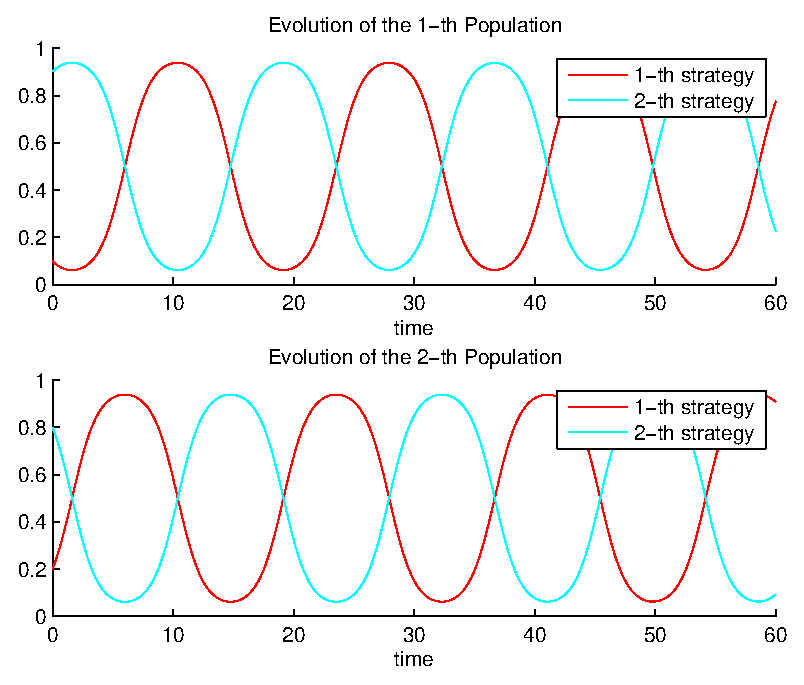
\includegraphics[width=\textwidth]{./images/test2_ev_rd.eps}
	  \caption{Evolution of the strategies in time.}
	  \label{fig:test2_ev_rd}
  \end{subfigure}
  \caption{Matching pennies game with replicator dynamics.}
  \label{fig:mp_game_rd}
\end{figure}



\begin{figure}[h]
  \centering
  \begin{subfigure}[b]{0.45\textwidth}
	  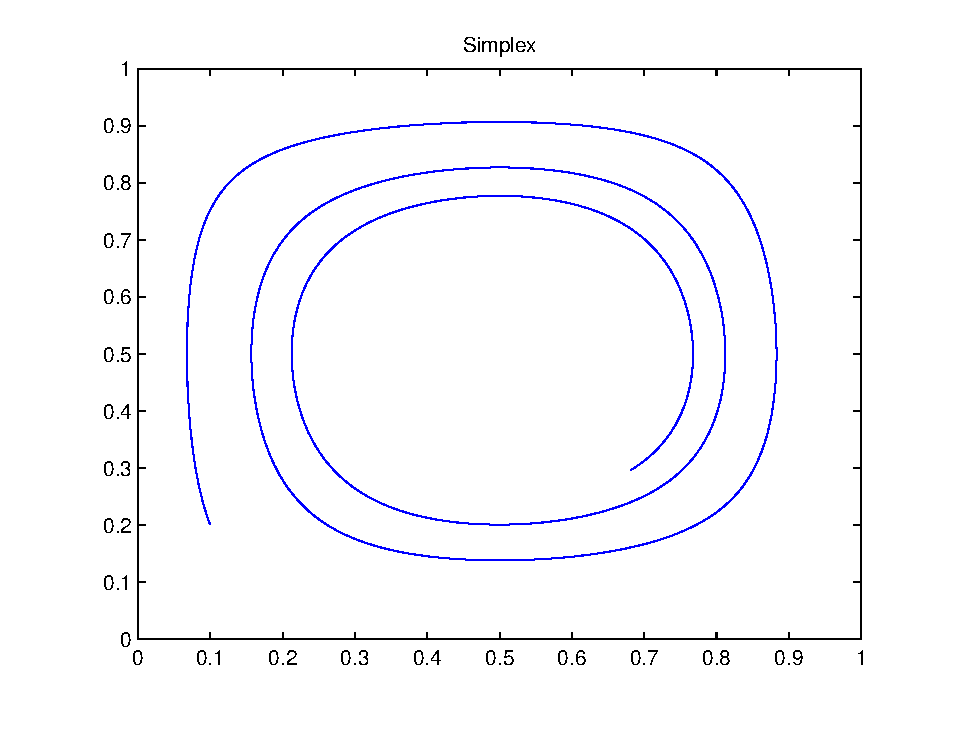
\includegraphics[width=\textwidth]{./images/test2_simplex_maynard_rd.eps}
	  \caption{Simplex.}
	  \label{fig:test2_simplex_maynard_rd}
  \end{subfigure}
  ~ 
  \begin{subfigure}[b]{0.45\textwidth}
	  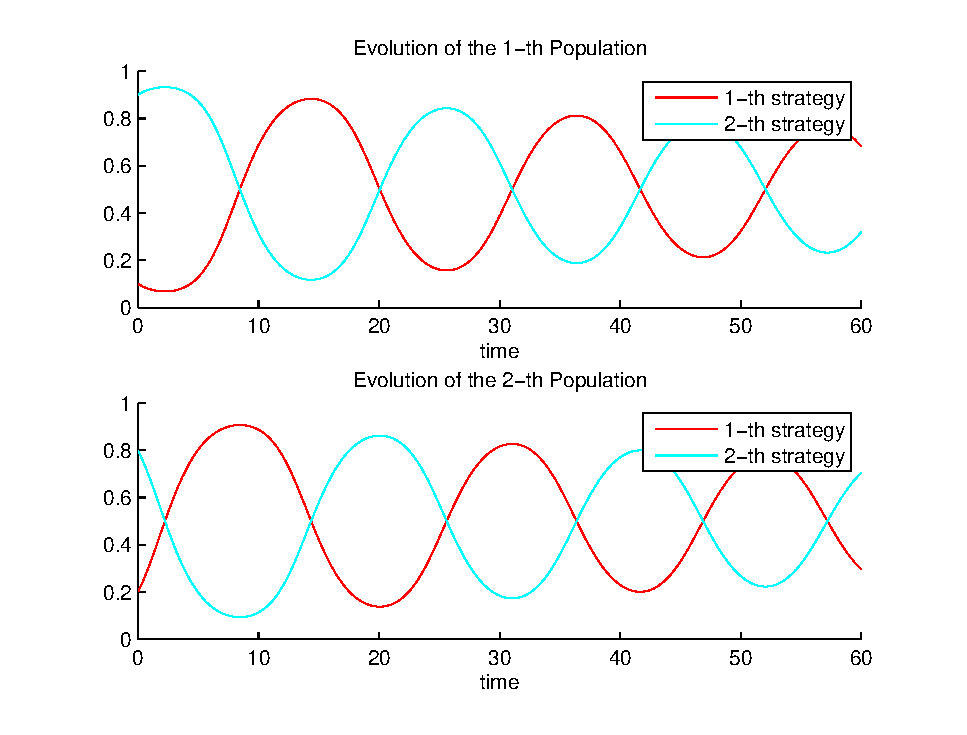
\includegraphics[width=\textwidth]{./images/test2_ev_maynard_rd.eps}
	  \caption{Evolution of the strategies in time.}
	  \label{fig:test2_ev_maynard_rd}
  \end{subfigure}
  \caption{Matching pennies game with Maynard replicator dynamics.}
  \label{fig:mp_game_maynard_rd}
\end{figure}



\begin{figure}[h]
  \centering
  \begin{subfigure}[b]{0.45\textwidth}
	  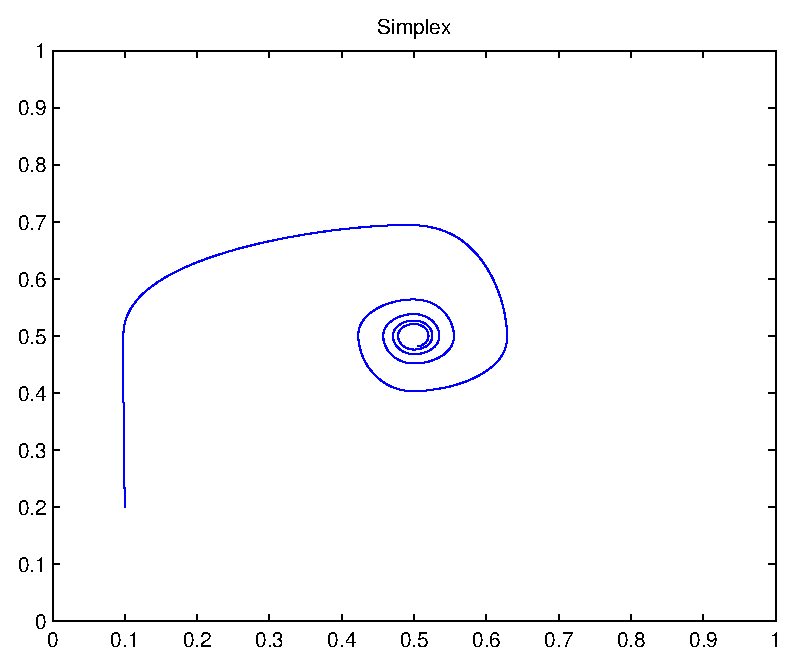
\includegraphics[width=\textwidth]{./images/test2_simplex_bnn.eps}
	  \caption{Simplex.}
	  \label{fig:test2_simplex_bnn}
  \end{subfigure}
  ~ 
  \begin{subfigure}[b]{0.45\textwidth}
	  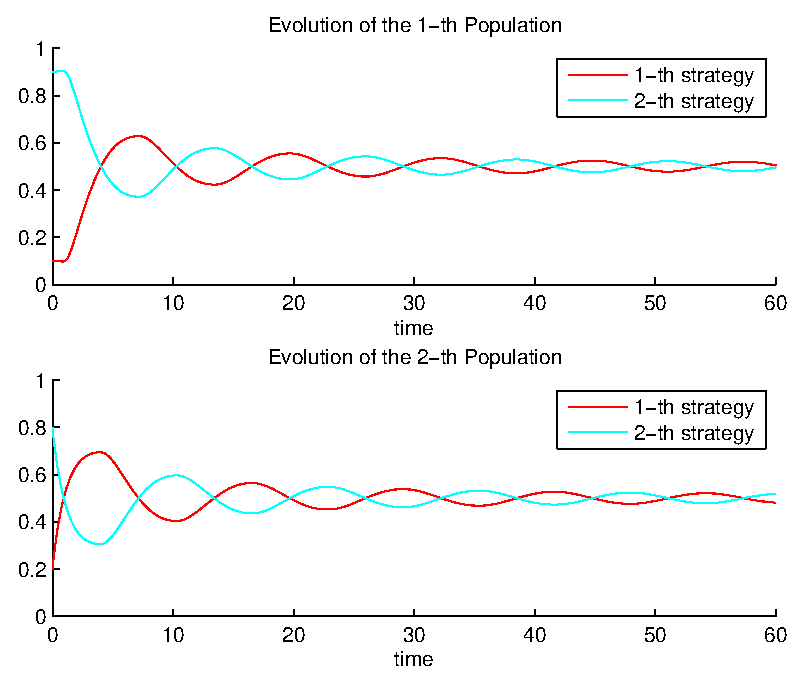
\includegraphics[width=\textwidth]{./images/test2_ev_bnn.eps}
	  \caption{Evolution of the strategies in time.}
	  \label{fig:test2_ev_bnn}
  \end{subfigure}
  \caption{Matching pennies game with BNN dynamics.}
  \label{fig:mp_game_bnn}
\end{figure}



\begin{figure}[h]
  \centering
  \begin{subfigure}[b]{0.45\textwidth}
	  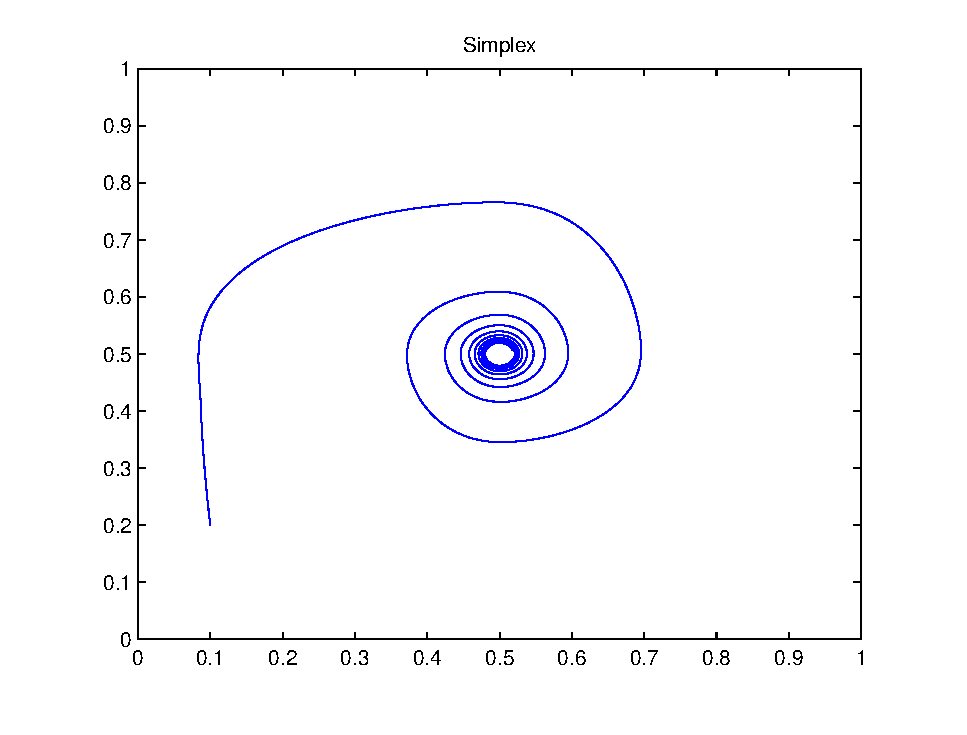
\includegraphics[width=\textwidth]{./images/test2_simplex_smith.eps}
	  \caption{Simplex.}
	  \label{fig:test2_simplex_smith}
  \end{subfigure}
  ~ 
  \begin{subfigure}[b]{0.45\textwidth}
	  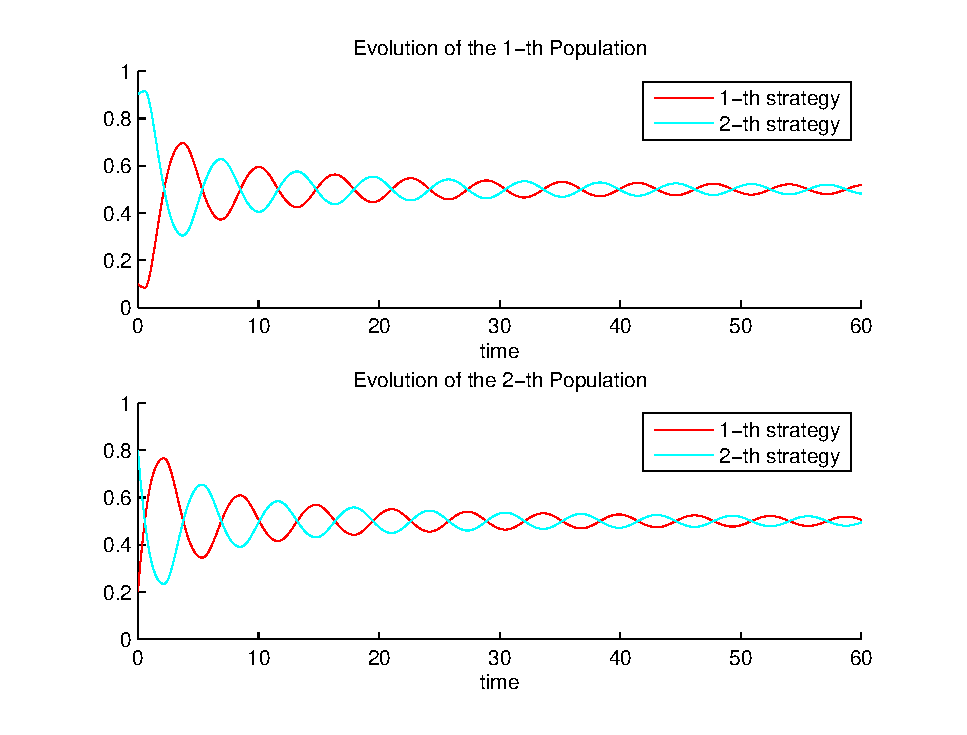
\includegraphics[width=\textwidth]{./images/test2_ev_smith.eps}
	  \caption{Evolution of the strategies in time.}
	  \label{fig:test2_ev_smith}
  \end{subfigure}
  \caption{Matching pennies game with Smith dynamics.}
  \label{fig:mp_game_smith}
\end{figure}



\begin{figure}[h]
  \centering
  \begin{subfigure}[b]{0.45\textwidth}
	  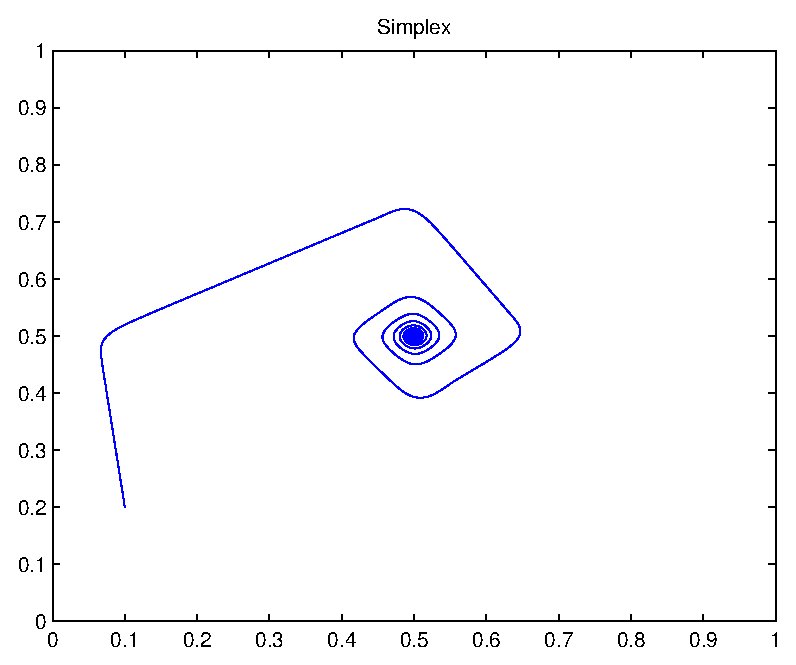
\includegraphics[width=\textwidth]{./images/test2_simplex_logit.eps}
	  \caption{Simplex.}
	  \label{fig:test2_simplex_logit}
  \end{subfigure}
  ~ 
  \begin{subfigure}[b]{0.45\textwidth}
	  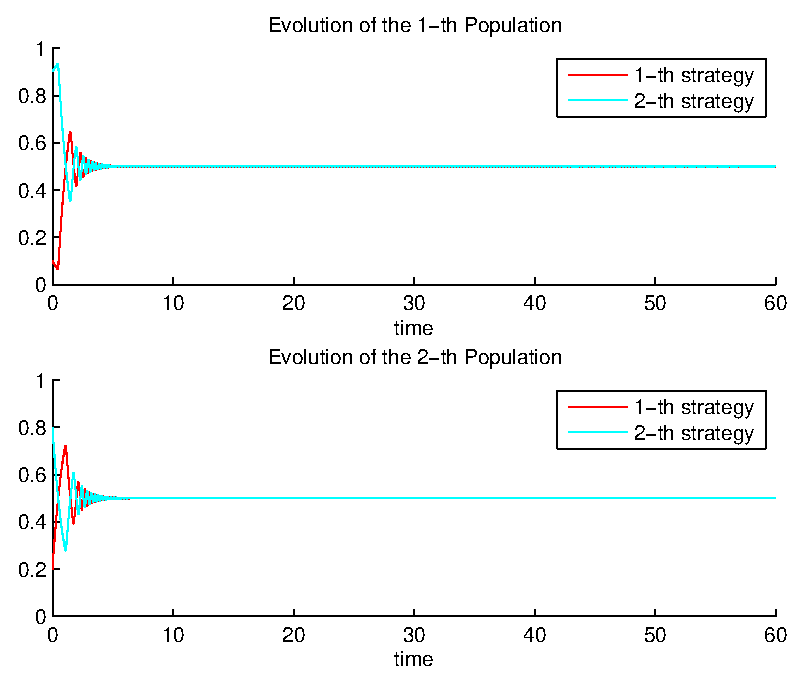
\includegraphics[width=\textwidth]{./images/test2_ev_logit.eps}
	  \caption{Evolution of the strategies in time.}
	  \label{fig:test2_ev_logit}
  \end{subfigure}
  \caption{Matching pennies game with Logit dynamics with $\eta=0.02$.}
  \label{fig:mp_game_logit}
\end{figure}



\newpage
\subsection{Demand response programs}

This is an example of multiple populations used to implement demand response programs in smart grids \cite{barreto2013design, barreto2014incentives}. In this case, we assume that each user must decide how to distribute its electricity usage along a day. Particularly, 
agents might have conflicting interests because they might impose externalities on the society through the price signals, i.e., the aggregated demand might affect the profit of agents. This conflict can be seen as a game between agents, in which each agent is selfish and  endeavors to maximize independently its own welfare. 

In this problem we model the daily electricity allocation problem as a multi-population game with nonlinear fitness functions. Particularly, each agent can implement an evolutionary dynamic to find the best distribution of resources. Note that when implemented locally by each user, the evolutionary dynamics lead to the global efficient equilibrium.

A particular feature of this problem is that the Nash equilibrium of the system is inefficient. Hence, 
we introduce an incentives scheme (indirect revelation mechanism) to maximize the aggregated surplus of the population.
The main feature of this mechanism is that it does not require private information from users, and employs a one dimensional message space to coordinate the demand profile of agents. These properties facilitate the distributed implementation of the mechanism. The mechanism entrusts the computation tasks among users, who should maximize its own utility function based the aggregated demand (that is calculated and broadcasted by a central agent). Thus, users avoid revelation of private information (e.g., preferences), but are required to report the aggregated consumption of their appliances during some time periods.







\subsubsection{Problem Formulation}



We consider a population composed by $N$ consumers defined as $\mathcal{V} = {1,\ldots.N}$. Also, let us divide a period of 24 hours in a set of $T$ time intervals denoted $\tau = \{\tau_1,\ldots,\tau_T\}$.
Formally, we define the set $\tau$ as a partition of $[0,24)$, where 
 $\cup_{t\in\{1,\ldots,T\}} \tau_t = \tau$ and $\cap_{t\in\{1,\ldots,T\}} \tau_t = \varnothing$.
%
Let $q_i^t$ be the electricity consumption of the $i\th$ user in the $t\th$ time interval. 
The daily electricity consumption of the $i\th$ user is represented by the vector $\bs{q}_i=[q_i^1,\ldots,q_i^T]^\top\in \Re_{\geq 0}^{T}$.
The population consumption at a given time $t$ is defined by the vector $\bs{q}^t = [q_1^t,, q_2^t\ldots,q_N^t]^\top\in \Re_{\geq 0}^{N}$.
On the other hand, the joint electricity consumption of the whole population is denoted by $\bs{q} = [\bs{q}_1^\top,
\ldots, \bs{q}_N^\top]^\top$. 
Without loss of generality, we assume that the electricity consumption of the $i\th$ user  satisfies $q_i^t\geq 0$,  in each time instant $t$.
A \emph{valuation function} $v_i^t(q_i^t)$ models the \emph{valuation} that the $i\th$ user gives to an electricity consumption of $q_i^t$ units in the $t\th$ time interval. Finally, let $p(\cdot):\Re\rightarrow\Re$ be the price of electricity charged to consumers. The aggregated consumption at a given time $t$ is defined as $||\bs{q}^t||_1 = \sum_{j=1}^N q_j^t$.
Moreover, a daily valuation is 
$v_i(\bs{q}_i)=\sum_{t=1}^T v_i^t(q_i^t),$
 where $t\in\{1,\ldots,T\}$.


 
 
 
Now, assuming  that the electricity generation cost is  the same for all $t$, we can express the profit function of each individual as
%
\begin{equation}\label{eq:u_i_}
 U_i(\bs{q}) = v_i(\bs{q}_i) - \sum_{t=1}^T q_i^t p\Big( \norm{\bs{q}^t}_1 \Big),
\end{equation}
%
where 
$p:\Re_+ \to \Re_+$ is the unitary price function.
The consumers welfare function is maximized by solving \cite{Johari09}
%
\begin{equation}\label{eq:opt_problem}
\begin{aligned}
& \underset{\bs{q}}{\text{maximize}}
& &  \sum_{i=1}^N U_i(\bs{q}) =  \sum_{i=1}^N\left( v_i(\bs{q}_i) - \sum_{t=1}^T q_i^t p\left( \norm{\bs{q}^t}_1 \right) \right) \\
& \text{subject to}
& & q_i^t \geq 0,  i =\{1,\ldots,N\}, t =\{1,\ldots,T\}.
\end{aligned}
\end{equation}



\subsubsection{Incentives}

The solution of the optimization problem in Eq.~(\ref{eq:opt_problem}) is inefficient in a strategic environment, i.e., when individuals are rational and selfish \cite{barreto2013design, Johari09}. In such cases, the analysis of strategic interactions among rational agents is made using game theory \cite{fudenberg98}.
In particular, the Nash equilibrium (a solution concept in game theory)  is sub-optimal, however, we can show that if we consider an added incentive to the individual cost function of each player, the Nash equilibrium of the game with incentives can be made efficient in the sense of Pareto \cite{barreto2013design, barreto2014incentives}. 

In particular, our DR scheme with incentives models the case when all agents keep their valuation of electricity to themselves, and have autonomous control their consumption. However, in order to incentive the agents to modify their behavior for the good of the population, the central entity sends them an incentive (e.g., a price signal or reward) to indirectly control their load.

Consider the new cost function for the $i^{th}$ agent:
\begin{equation}\label{eq:game2}
W_i(q_i,\bs{q}_{-i}) 
%=  W_i(\bs{q}) + I_i(\bs{q}) 
= v_i(q_i) -  q_i p\left( \norm{\bs{q}^t}_1 \right) + I_i(\bs{q}) .
%\vspace{-.3cm}
\end{equation}
where incentives are of the form:
\begin{equation}\label{eq:I_i}
I_i(\bs{q}) = \left( \norm{\bs{q}_{-i}^t}_1\right) \left( h_i(\norm{\bs{q}_{-i}})  - p\left( \norm{\bs{q}^t}_1 \right) \right).
%\vspace{-.3cm}
\end{equation}


The form of this incentive is inspired in the 
Vickrey-Clarke-Groves mechanism and the  Clarke pivot rule \cite{AlgorithmicG}.
%
We assign incentives according to the contribution made by an agent 
to the society. In particular, the function $h_i:\Re \to \Re$ is a design parameter that estimates the externalities introduced by each individual.
%\begin{equation}\label{eq:h}
%h_i(\bs{\bs{q}}_{-i})=
%p\Big( \sum\nolimits_{j\neq i} q_j + f(\bs{\bs{q}}_{-i}) \Big),
%\end{equation}
%were $f(\cdot)$ might be a linear function. 
It can be shown that these incentives can lead to an optimal equilibrium in a strategic environment.
In this DR approach we consider that the utility sends a two dimensional signal to each customer, namely $(q,I_i)$ and each customer responds with some consumption $q_i$. 
Note that the incentives modify the price paid by each user according to their relative consumption. However, two different users receive different incentives as long as their consumption are different.

\subsubsection{Simulations}




In this section, we illustrate some ideas of efficiency and the decentralized implementation of the incentives mechanism. We select some functions used previously in the literature. On the one hand, we define the family of valuation functions as 
\begin{equation}\label{eq:valuation_sim}
 v(\bs{q}^k,\alpha_i^k) = v_i^k (q_i^k) = \alpha_i^k \log(1+q_i^k)
\end{equation}
where $\alpha_i^k>0$ is the parameter that characterizes the valuation of the  $i\th$ agent at the $k\th$ time instant.
On the other hand, the generation cost function is defined as 
%
\begin{equation}\label{eq:cost_sim}
 C(\|\bs{q}\|_1) = \beta ({\|\bs{q}\|_1})^2 + b {\|\bs{q}\|_1},
\end{equation}
and the unitary price function is
%
\begin{equation}\label{eq:p_sim}
 p(\|\bs{q}\|_1) = \frac{C(\|\bs{q}\|_1)}{\|\bs{q}\|_1} = \beta \|\bs{q}\|_1 + b.
\end{equation}
%
Note that the generation cost only depends on the aggregated consumption, not on the time of the day. Furthermore, 
%
the fitness function of the system with incentives is
%
\begin{equation}\label{eq:fitness_without_i_sim}
F_i^k( \bs{q}^k)  =  \frac{\alpha_i^k }{1+q_i^k}
 - 2\beta \left( \sum_{j=1}^N q_j^k  \right).
 \end{equation}


The evolution of utility, demand, and incentives for different dynamics is shown in Figs.~\ref{fig:dynamics_u} and \ref{fig:dynamics_i}. Note that despite using the same initial condition, the evolution of the system is different with each dynamical model. In particular, BNN and Smith dynamics converge faster to the  optimum, in contrast with the Logit and replicator dynamics. 
This is achieved by means of a fast decrease in the power consumption. 

\begin{figure}[hbt]
 \centering
 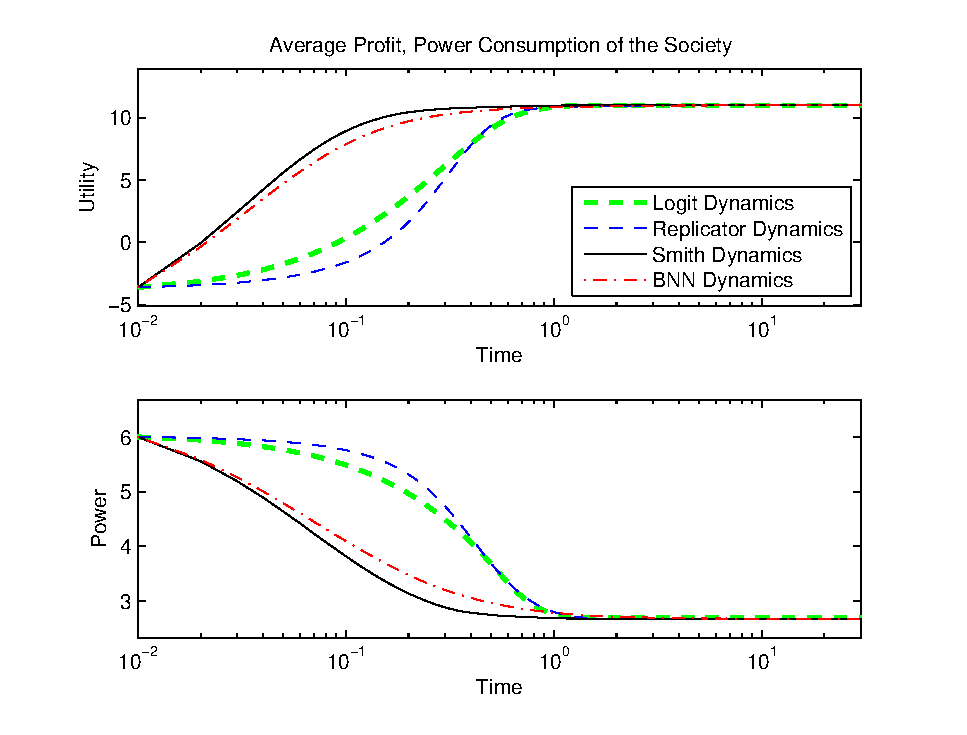
\includegraphics[width=.75\textwidth]{./images/evolution_u.eps}
 \caption{Evolution of profit and costs for four different dynamics.}
 \label{fig:dynamics_u}
\end{figure}


\begin{figure}[hbt]
 \centering
 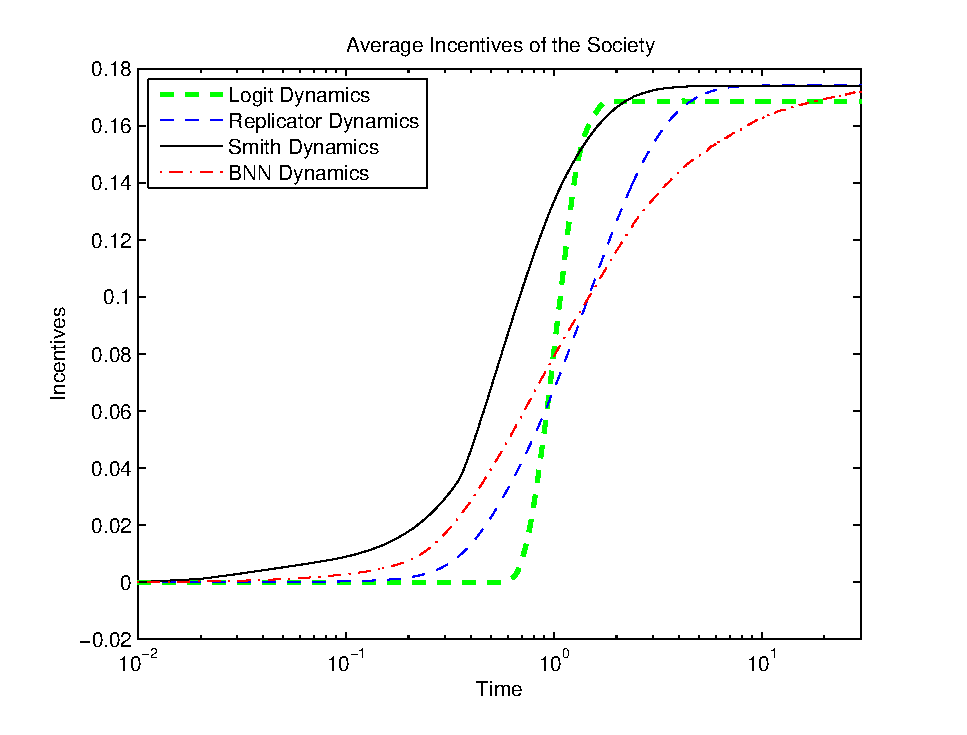
\includegraphics[width=.75\textwidth]{./images/evolution_i.eps}
 \caption{Evolution of the incentives with four different dynamics.}
 \label{fig:dynamics_i}
\end{figure}



Incentives in Fig.~\ref{fig:dynamics_i} show that, in the long run, all dynamics converge to the same level of incentives. Particularly, Smith dynamics requires more incentives during all time, except for logit dynamics, which has a sudden increase in the incentives close to the equilibrium point. 

In Fig.~\ref{fig:dynamics_i} it is not clear which dynamical model moves the state of the system to the optimal equilibrium using less resources. To answer this question, we simulate the total amount of incentives used by each model.
Thus, let us define the aggregated incentives in a society in a particular time $t$ as
\begin{equation}
 I_d (t) = \sum_{i\in\mathcal{P}} \frac{1}{|S|} \sum_{k\in S} I_i \left( \bs{q}^k (t) \right).
\end{equation}
Now, the total accumulated incentives from $t_0$ to $t$ is defined as 
\begin{equation}
 \varPhi_d (t) = \int_{t_0}^t I_d (\tau) d\tau.
\end{equation}
Thus, $\varPhi_d (t)$ gives a measurement of the total amount subsidies required by the system with dynamic $d$, in the time interval  $[t_0, t]$.
In this case we do not have a reference to compare the subsidies requirements of each evolutionary dynamic. Hence, we compare the subsidies requirements with the average requirements of all the dynamics implemented. 
%
In order to see which dynamic requires more resources, we plot the cumulative resources required by each dynamic relative to the average.
Hence, we define the cumulative incentives as 
%
\begin{equation}
CI_d = \frac{ \varPhi_d (t) }{ \sum_{d\in \mathcal{D}} \varPhi_d (t) }.
\end{equation}
%
Fig.~\ref{fig:integral} shows the results of the simulation of the relative subsidies required by each model of evolutionary dynamics.
%



Smith dynamics requires much more resources during all the time stamp, but is particularly high during the first stages, while logit has the lower incentives requirements. However, BNN has the lower incentives in long run.

\begin{figure}[hbt]
 \centering
 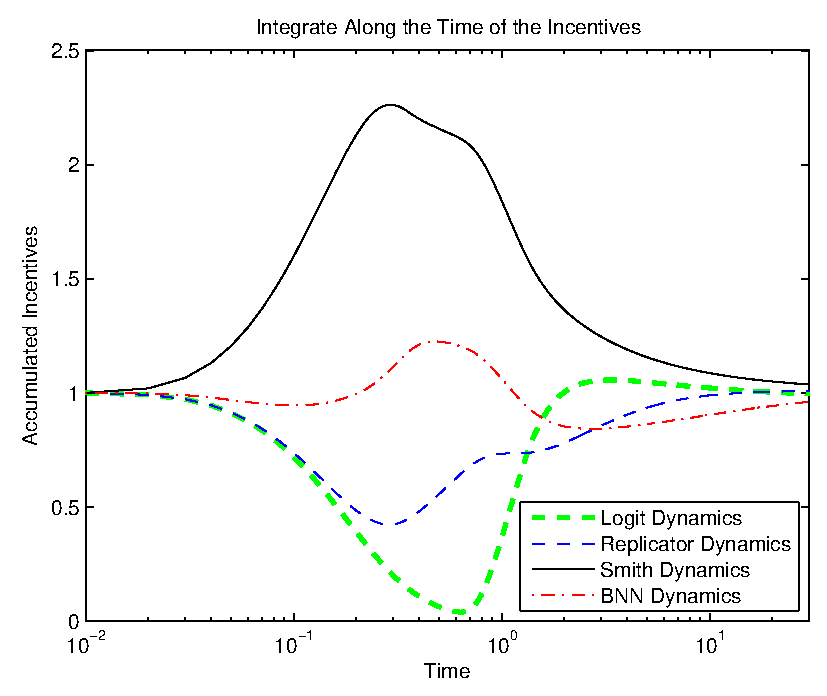
\includegraphics[width=.75\textwidth]{./images/accumulated_i.eps}
 \caption{Accumulated incentives during the evolution of the algorithm.}
 \label{fig:integral}
\end{figure}



Fig. \ref{fig:final_state} shows the final demand profile of each agent. Note that the final state corresponds to the state of each population at the equilibrium.

\begin{figure}[hbt]
 \centering
 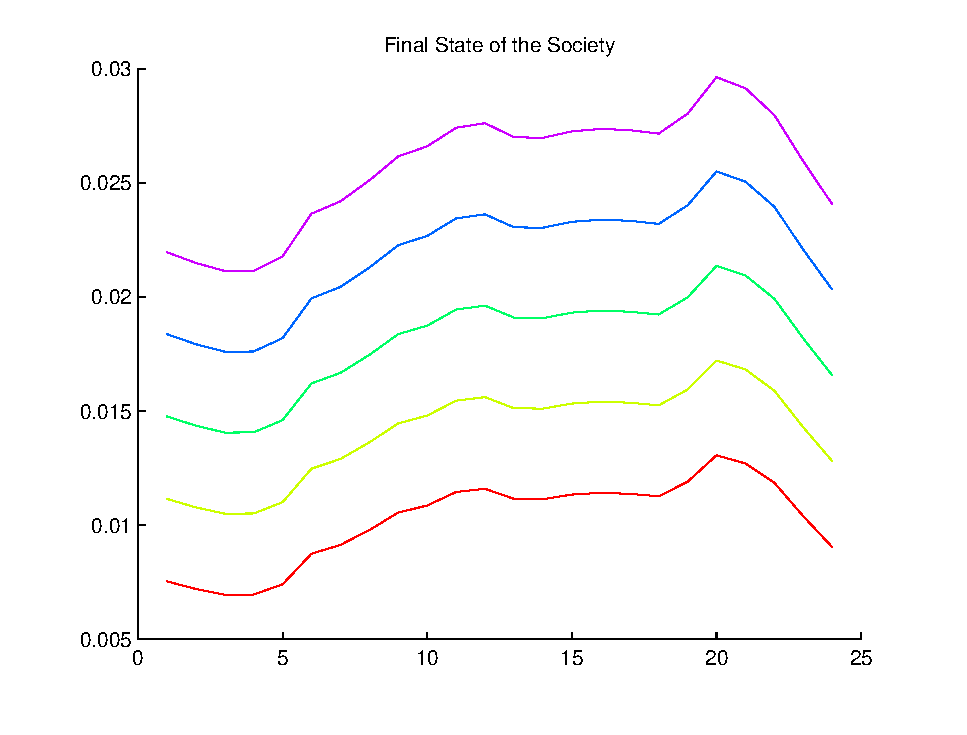
\includegraphics[width=.75\textwidth]{./images/final_state.eps}
 \caption{Final demand profile of each agent.}
 \label{fig:final_state}
\end{figure}






\iffalse

\section{Designing games}

In the previous section we show some examples of strategical situations that can be analyzed with game theory. In these cases, the structure of the game is given by the problem. However, we can modify the fitness function of each player in order to solve an optimization problem.

For example, let us consider the following optimization problem:

\begin{equation}\label{eq:opt_problem}
\begin{aligned}
& \underset{x}{\text{maximize}} 
& & \sum_{i=1}^N U_i(x_i)  - C(|x|)\\
& \text{subject to}
& & 0 \leq q_i \geq m,  i =\{1,\ldots, N\}.
\end{aligned}
\end{equation}

This can be seen as a problem of allocating a finite resource to maximize a utility function. 

Note that there are $N$ agents with that give a valuation $v_i(x_i)$ to the resource $x_i$.

However, the cost of assigning the resource is $C(|x|)$ .

The cost of assigning the resource might be distributed among the population. 

Let us consider the following example:


\begin{equation}
U_i(x_i) =   \alpha_i  log(1+x_i) 
\end{equation}

\begin{equation}
C(z) = \beta z^2 + b z 
\end{equation}

define fitness functions as 

\begin{equation}
f_i(x_1, x_2) = \frac{\alpha_i}{1+x_i} - 2 \beta |x| - b 
\end{equation}










------------

With a finite population the time specifies the number of iterations.

There might be different populations!!!

How do we define the state vector???




\fi












\bibliographystyle{plain}
\bibliography{references}




\iffalse


      
\begin{figure}[htb]
 \includegraphics[1\textwidth]{./images/}
 \caption{}
 \label{fig:}
\end{figure}




test1_ev_bnn.eps         test1_simplex_rd.eps     test2_simplex_bnn.eps
test1_ev_logit.eps       test1_simplex_smith.eps  test2_simplex_logit.eps
test1_ev_rd.eps          test2_ev_bnn.eps         test2_simplex_rd.eps
test1_ev_smith.eps       test2_ev_logit.eps       test2_simplex_smith.eps
test1_simplex_bnn.eps    test2_ev_rd.eps
test1_simplex_logit.eps  test2_ev_smith.eps
\fi

\end{document}










%

\section{Revision Protocols}


\subsection{Pairwise Proportional Imitation}

The $i\th$ agent observes an opponent $j$ at random. Then might change its strategy if  its opponent has a greater fitness. The rate change is 

\begin{equation}
\rho_{ij}(\pi, x) = \frac{x_j}{m} [\pi_j - \pi_i]_+
\end{equation}

In this case, $x_j$ need not be observed. This protocol lead to replicator dynamics.


	

\subsection{Comparison of the Average Payoff}

The $i\th$ agent selects a strategy at random and might switch to it if that strategy has payoff above the average. The agent switch strategy with probability proportional to the excess payoff

\begin{equation}
\rho_{ij}(\pi, x) = \left[ \pi_j - \frac{1}{m} \sum_{k\in S} x_k \pi_k \right]_+
\end{equation}

This protocol lead to BNN dynamics.

\subsection{Pairwise Comparison}

$i\th$ agent selects a strategy at random. If the opponent has a higher fitness, the the agent switch strategy with probability proportional to

\begin{equation}
\rho_{ij}(\pi, x) = \left[ \pi_j - \pi_i \right]_+
\end{equation}

This protocol leads to Smith dynamics.



\subsection{Logit Choice}

The $i\th$ agent selects a strategy at random and change its strategy with a probability proportional to 

\begin{equation}
\rho_{ij}(\pi) = \frac{ \exp(\pi_j \eta^{-1} ) }{ \sum_{k \in S} \exp(\pi_k \eta^{-1} ) }
\end{equation}

This protocol leads to Logit dynamics.







%\subsection{Examples of games Population of small agents}




The following are some examples of games with small number of agents. 
We implement the rock-paper-scissors game. This game has only one population with three strategies, denoted $x = [x_1, x_2, x_3]^\top$. The fitness function is defined as $F(x)=Ax$, where A is equal to 
\begin{equation}
  A = \begin{pmatrix}
  0  & -1 &  1 \\
  1  &  0 & -1 \\
  -1 &  1 & 0
  \end{pmatrix}
\end{equation}

We implement four revision protocols, namely, proportional imitation, comparison to average, pairwise comparison, and logit choice. Fig. \ref{fig:finite1} to \ref{fig:finite4} show the evolution of the society with each revision protocol.

Simulations are made with $200$ agents and 10000 iterations.
The evolution might take place in days, months, years.




\begin{figure}
  \centering
  \begin{subfigure}[b]{0.45\textwidth}
	  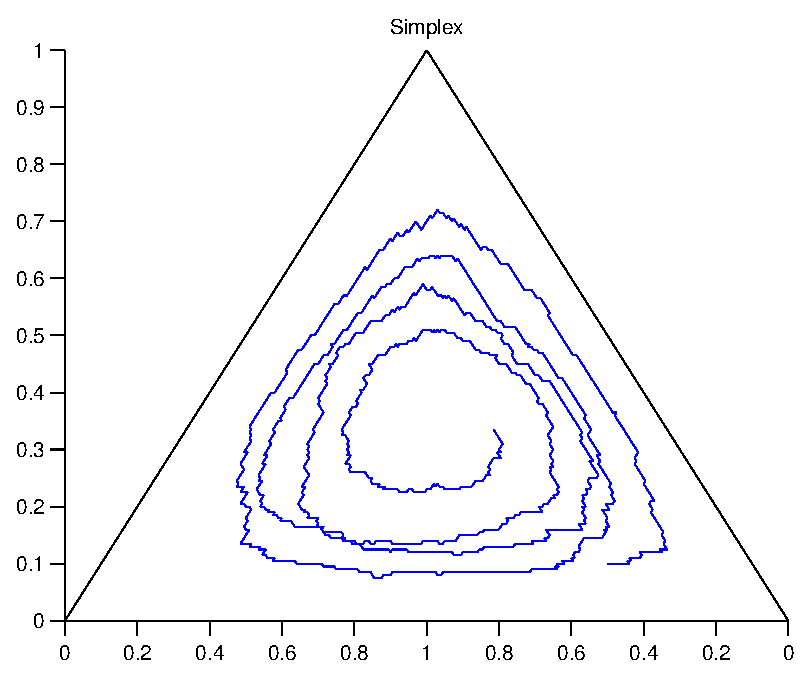
\includegraphics[width=\textwidth]{./images/test_finite_proportional_imitation.eps}
	  \caption{Simplex.}
	  \label{fig:finite1_simplex}
  \end{subfigure}
  ~ 
  \begin{subfigure}[b]{0.45\textwidth}
	  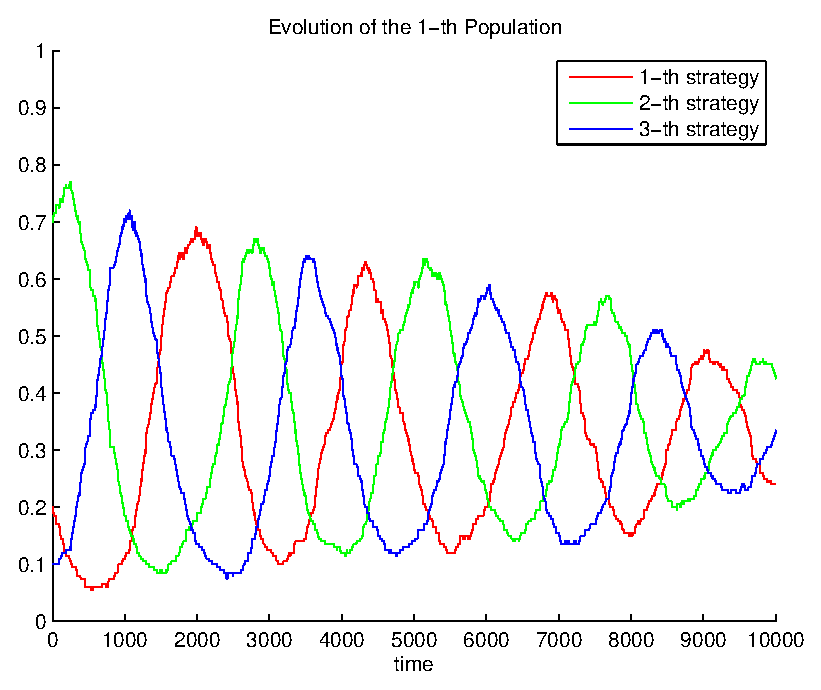
\includegraphics[width=\textwidth]{./images/test_finite_proportional_imitation_ev.eps}
	  \caption{Evolution of the strategies in time.}
	  \label{fig:finite1_ev}
  \end{subfigure}
  \caption{Rock-paper-scissors game with proportional imitation revision protocol (Replicator dynamics with large number of agents).}
  \label{fig:finite1}
\end{figure}


\begin{figure}
  \centering
  \begin{subfigure}[b]{0.45\textwidth}
	  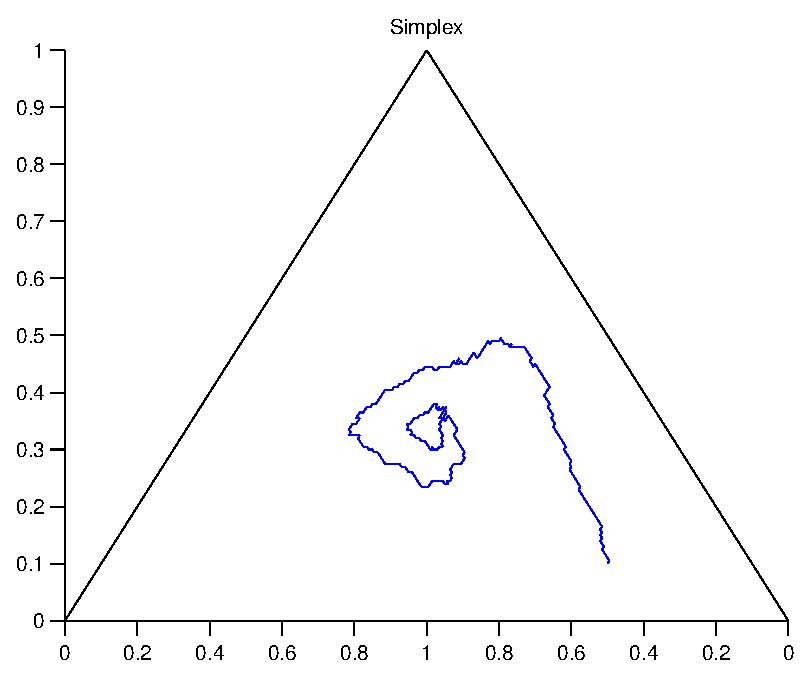
\includegraphics[width=\textwidth]{./images/test_finite_comparison2average.eps}
	  \caption{Simplex.}
	  \label{fig:finite2_simplex}
  \end{subfigure}
  ~ 
  \begin{subfigure}[b]{0.45\textwidth}
	  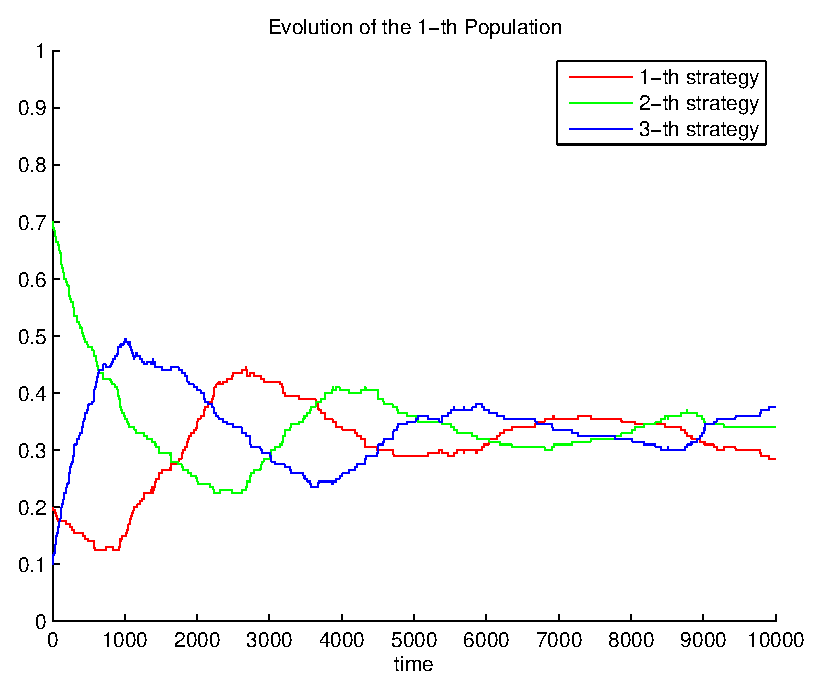
\includegraphics[width=\textwidth]{./images/test_finite_comparison2average_ev.eps}
	  \caption{Evolution of the strategies in time.}
	  \label{fig:finite2_ev}
  \end{subfigure}
  \caption{Rock-paper-scissors game with comparison to average revision protocol (BNN dynamics with large number of agents).}
  \label{fig:finite2}
\end{figure}


\begin{figure}
  \centering
  \begin{subfigure}[b]{0.45\textwidth}
	  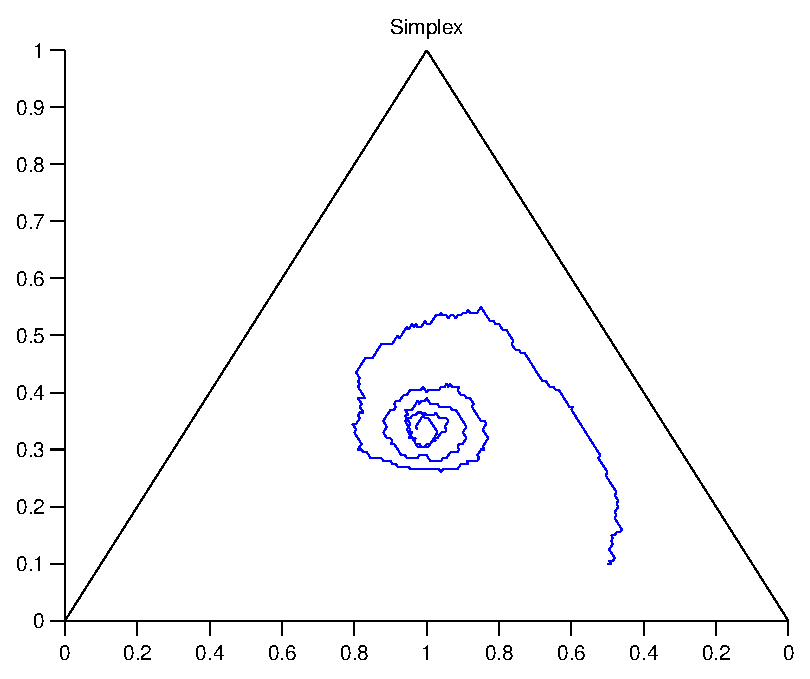
\includegraphics[width=\textwidth]{./images/test_finite_pairwise_comparison.eps}
	  \caption{Simplex.}
	  \label{fig:finite3_simplex}
  \end{subfigure}
  ~ 
  \begin{subfigure}[b]{0.45\textwidth}
	  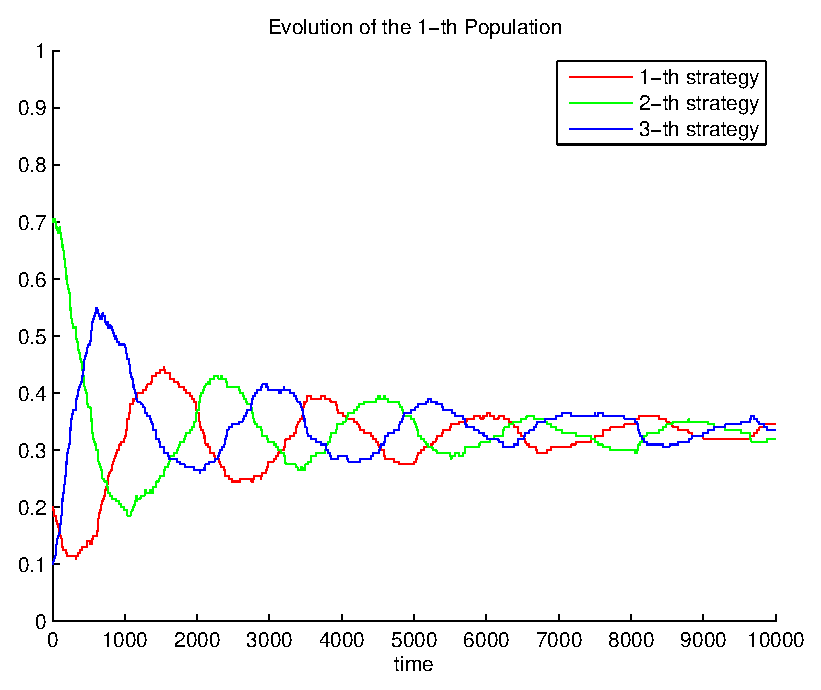
\includegraphics[width=\textwidth]{./images/test_finite_pairwise_comparison_ev.eps}
	  \caption{Evolution of the strategies in time.}
	  \label{fig:finite3_ev}
  \end{subfigure}
  \caption{Rock-paper-scissors game with pairwise comparison revision protocol (Smith dynamics with large number of agents).}
  \label{fig:finite3}
\end{figure}


\begin{figure}
  \centering
  \begin{subfigure}[b]{0.45\textwidth}
	  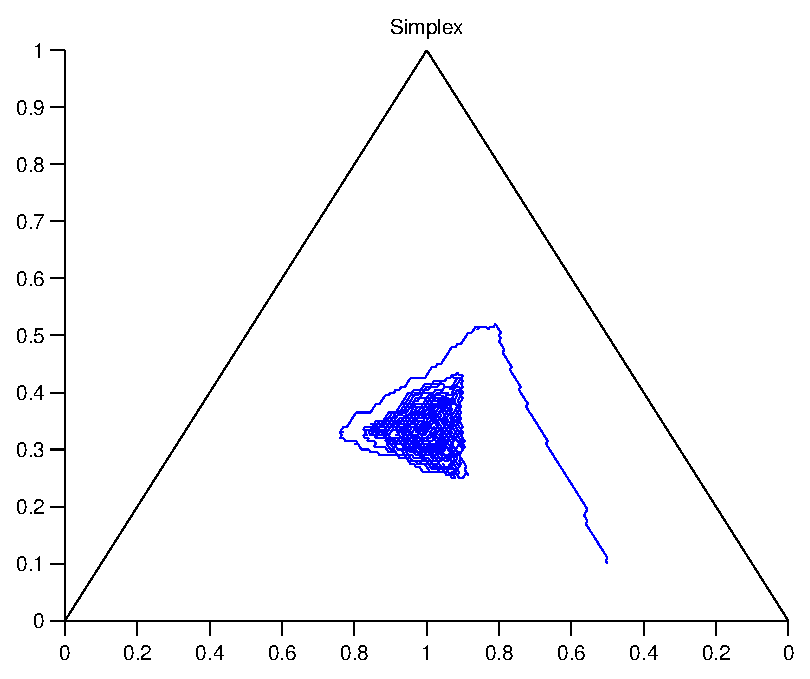
\includegraphics[width=\textwidth]{./images/test_finite_logit_choice.eps}
	  \caption{Simplex.}
	  \label{fig:finite4_simplex}
  \end{subfigure}
  ~ 
  \begin{subfigure}[b]{0.45\textwidth}
	  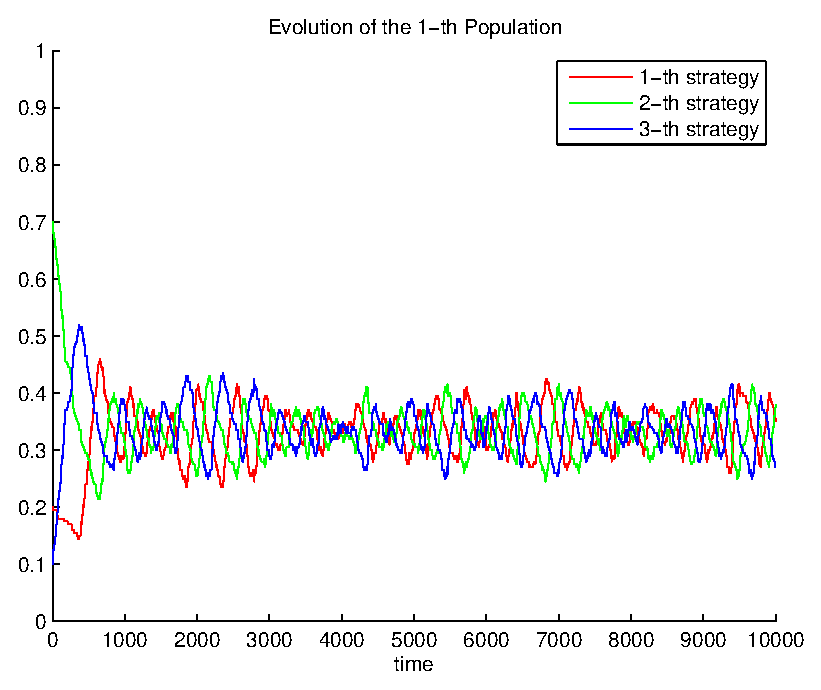
\includegraphics[width=\textwidth]{./images/test_finite_logit_choice_ev.eps}
	  \caption{Evolution of the strategies in time.}
	  \label{fig:finite4_ev}
  \end{subfigure}
  \caption{Rock-paper-scissors game with logit choice revision protocol ( dynamics with large number of agents).}
  \label{fig:finite4}
\end{figure}






% 
 
\section{Revision Protocols and Evolutionary Dynamics}\label{sec:protocols}
 
 
In this section we introduce four revision protocols, that lead to the evolutionary dynamics \emph{logit dynamics} (Logit), \emph{replicator dynamics} (RD), \emph{Brown-von Neumann-Nash dynamics} (BNN), and \emph{Smith dynamics} (Smith). These dynamics belong to the families of \emph{perturbed optimization}, \emph{imitative dynamics}, \emph{excess payoff dynamics}, and \emph{pairwise comparison dynamics}, respectively \cite{hofbauer2001nash, sandholm_book}. 
 
 
 
 
 
 
 \subsection{Pairwise Proportional Imitation (Replicator Dynamics)}

With a revision opportunity the $i\th$ agent observes an opponent $j$ at random. Then it might change its strategy if  its opponent has a greater fitness. The rate change is 
%
\begin{equation}
\rho_{ij}^p(\pi^p, x^p) = \frac{1}{m^p} [\pi_j^p - \pi_i^p]_+,
\end{equation}
where the $[\cdot]_+:\Re \leftarrow \Re_{\geq0}$ represents the positive part, defined as $[ x ]_+ \equiv \max\{ 0, x \}$.
This protocol leads to the \emph{replicator dynamics} defined as
\begin{equation}\label{eq:replicator}
\dot{x}_i^p = x_i^p \, \hat{F}_i^p \left( x \right),
\end{equation}
where $\hat{F}_i^p$ is the excess payoff to strategy $i\in S^p$, which is defined as   
\begin{equation}
\hat{F}_i^p (x) =  F_i^p(x) - \bar{F}^p(x),
\end{equation}
and $\bar{F}^p(x)$ is the average payoff the population $p$, i.e., 
\begin{equation}
 \bar{F}^p(x) = \frac{1}{m^p} \sum_{j \in S^p} x_j^p F_j^p(x).
\end{equation}



\subsubsection*{Algorithm}

\begin{algorithm}[H]
\SetKwInOut{Input}{input}\SetKwInOut{Output}{output}

 \Input{Society's state $x$}
 \Output{State update $\dot{x}$}
 \BlankLine
 
 \For{ $ p \leftarrow 1 $ \KwTo $P$ } {
  $ F^p \leftarrow fitness(x, p)$\;
  $ \bar{F}^p \leftarrow \frac{1}{m^p} (F^p)^\top x^p$\;
  $ \hat{F}^p \leftarrow F^p - \boldsymbol{1} \bar{F}^p$\;
  $ \dot{x}^p \leftarrow \hat{F}^p \odot x^p \frac{1}{m^p} $\; 
 }
\end{algorithm}
%
The running time of the algorithm is $T_{rd}(n, P) = O( P (  T_{f}(n,P) + n) ) $, where $T_{f}(n,P)$ is the time required to calculate the fitness vector of a population.








\subsection{Comparison to the Average Payoff (Brown-von Neumann-Nash Dynamics (BNN))}

With a revision opportunity the $i\th$ agent selects a strategy at random and might switch to it if that strategy has a payoff above the average. The agent switch strategy with probability proportional to the excess payoff
%
\begin{equation}
\rho_{ij}^p(\pi^p, x^p) = \left[ \pi_j^p - \frac{1}{m^p} \sum_{k\in S^p} x_k^p \pi_k^p \right]_+,
\end{equation}

This protocol leads to \emph{Brown-von Neumann-Nash dynamics}, defined as 
\begin{equation}\label{eq:bnn}
 \dot{x}_i^p = \left[ \hat{F}_i^p \left( \bs{x} \right) \right]_+ - x_i^p  \sum_{j \in S^p} \left[ \hat{F}_j^p \left( \bs{x} \right) \right]_+.
\end{equation}



\subsubsection*{Algorithm}

\begin{algorithm}[H]
\SetKwInOut{Input}{input}\SetKwInOut{Output}{output}

 \Input{Society's state $x$}
 \Output{State update $\dot{x}$}
 \BlankLine
 
 \For{ $ p \leftarrow 1 $ \KwTo $P$ } {
  $ F^p \leftarrow fitness(x, p)$\;
  $ \bar{F}^p \leftarrow \frac{1}{m^p} (F^p)^\top x^p$\;
  $ \hat{F}^p \leftarrow \max\{F^p - \boldsymbol{1} \bar{F}^p, \boldsymbol{0}\}$\;
  $ \dot{x}^p \leftarrow \hat{F}^p - (\boldsymbol{1}^\top \hat{F}^p) \odot x^p \frac{1}{m^p} $\;
 }
\end{algorithm}
%
The running time is $T_{BNN}(n,P) = O( P (  T_{f}(n,P) + n) ) $.






\subsection{Pairwise Comparison (Smith Dynamics)}

With a revision opportunity the $i\th$ agent selects a strategy at random. If the opponent has a higher fitness, the the agent switch strategy with probability proportional to
\begin{equation}
\rho_{ij}(\pi, x) = \left[ \pi_j - \pi_i \right]_+
\end{equation}
This protocol leads to \emph{Smith dynamics} that are defined as 
%
\begin{equation} 
\dot{x}_i^p  = \sum_{\gamma \in S^p} x_\gamma^p  \left[ F_i^p \left( \bs{x} \right) - F_\gamma^p \left( \bs{x} \right) \right]_+ 
%%\\
- x_i^p  \sum_{\gamma \in S^p} \left[ F_\gamma^p ( \bs{x}) - F_i^p( \bs{x} ) \right]_+.
\label{eq:smith}
\end{equation}


\subsubsection*{Algorithm}

Here we present two algorithms. 
The first one has time complexity  $O(P(T_f(n, P)+ n^2 ))$. This algorithm is implemented as `smith.m'. A characteristic of this implementation is that might be faster under some conditions, because Matlab is optimized to operate with matrices (see more in Section \ref{sec:running_time}).

\begin{algorithm}[H]
\SetKwInOut{Input}{input}\SetKwInOut{Output}{output}

 \Input{Society's state $x$}
 \Output{State update $\dot{x}$}
 \BlankLine
 \For{ $ p \leftarrow 1 $ \KwTo $P$ } {
  $ F^p \leftarrow fitness(x, p)$\;
  $A \leftarrow \boldsymbol{1} {F^p}^\top$\;
  $M \leftarrow \max(\boldsymbol{0}_{n\times n}, A-A^\top)$\;
  
  $F_{sum}^p \leftarrow M \boldsymbol{1}$\;
  $F_{avg}^p \leftarrow \frac{1}{m^p} x^\top \, M$\;

  $ \dot{x}^p \leftarrow F_{avg}^p - F_{sum}^p \odot x^p \frac{1}{m^p}$\;
 }
\end{algorithm}


Below we present an alternative algorithm that might be faster for large number of strategies.
In this case we order the strategies in increasing order of fitness and then calculate the strategy's fitness difference (only the ones that are positive). This allow us to reduce the number of operations. The running time of this algorithm is $T_{smith}(n,p) = O(P(T_f(n, P)+ n\log(n) ))$. This algorithm is implemented as `smith\_b.m'.


\begin{algorithm}[H]
\SetKwInOut{Input}{input}\SetKwInOut{Output}{output}

 \Input{Society's state $x$}
 \Output{State update $\dot{x}$}
 \BlankLine
 \For{ $ p \leftarrow 1 $ \KwTo $P$ } {
  $ F^p \leftarrow fitness(x, p)$\;
  $A \leftarrow$ Fitness functions ordered in ascending order\;
  $B \leftarrow$ Strategies ordered in ascending order by their fitness  \;
  
  $A_{sum} \leftarrow \boldsymbol{1}^\top A$\;
  $A_{avg} \leftarrow 0$\;
  $x_{ord} \leftarrow x(B)\frac{1}{m^p} $\;
  $x_{cum} \leftarrow 0$\;
  
  \For{ $i \leftarrow 1$ \KwTo $n^p$ }{
    $k \leftarrow B(i)$\;
    $A_{sum} \leftarrow A_{sum} - A(i)$\:
   
    
    $\Gamma_a^p[k] \leftarrow A(i) x_{cum} - A_{avg}$\;
    $\Gamma_b^p[k] \leftarrow A_{sum} - A(i) (n-i) $\;
    
    $A_{avg} \leftarrow A_{avg} + A(i) x_{ord}(i)$\;
    $x_{cum} \leftarrow x_{cum} + x_{ord}(i)$\;
 
  }
  $ \dot{x}^p \leftarrow \Gamma_a^p - \Gamma_b^p \odot x^p \frac{1}{m^p}$\;
 }
\end{algorithm}




\subsection{Logit Choice}

With a revision opportunity the $i\th$ agent selects a strategy at random and change its strategy with a probability proportional to 

\begin{equation}
\rho_{ij}(\pi) = \frac{ \exp(\pi_j \eta^{-1} ) }{ \sum_{k \in S} \exp(\pi_k \eta^{-1} ) }
\end{equation}

This protocol belong to target dynamics and with a large population results in the following dynamics
\begin{equation}\label{eq:logit}
 \dot{x}_i^p = \frac{ \exp\left(\eta^{-1} F_i^p (\bs{x}) \right) }{ \sum_{\gamma \in S^p} \exp\left(\eta^{-1} F_\gamma^p (\bs{x}) \right) }, \, \, \eta>0,
\end{equation}
known ad \emph{Logit dynamics}. 



\subsubsection*{Algorithm}

\begin{algorithm}[H]
\SetKwInOut{Input}{input}\SetKwInOut{Output}{output}

 \Input{Society's state $x$}
 \Output{State update $\dot{x}$}
 \BlankLine
 
 \For{ $ p \leftarrow 1 $ \KwTo $P$ } {
  $ F^p \leftarrow fitness(x, p)$\;
  $ \bar{F}^p \leftarrow \frac{1}{m^p} (F^p)^\top x^p$\;
  $ \tilde{F}^p \leftarrow \exp( F^p \eta^{-1} )$\;
  $ \Gamma \leftarrow \boldsymbol{1}^\top \tilde{F}^p $\;
  $ \dot{x}^p \leftarrow \frac{\tilde{F}^p}{\Gamma} - x^p $\;
 }
\end{algorithm}

The running time is $T_{logit}(n,P) = O( P (  T_{f}(n,P) + n) ) $.



\iffalse
\subsection{Maynard Smith Replicator}

\begin{equation}
\dot{x}_i = \frac{ x_i F_i }{ \bar{F}(x) } - x_i
\end{equation}
\fi





\iffalse

\subsection{Examples}
We show examples of two games that have different number of populations and strategies per population.

\subsubsection{Rock-paper-scissors game}
We implement the rock-paper-scissors game. This game has only one population with three strategies, denoted $x = [x_1, x_2, x_3]^\top$. The fitness function is defined as $F(x)=Ax$.

Fig.\ref{fig:rpc_game_rd} to \ref{fig:rpc_game_logit} show the evolution of the social state. Note that the evolution of the dynamical approximation resembles the behavior of the system with small number of agents.


\begin{figure}
  \centering
  \begin{subfigure}[b]{0.45\textwidth}
	  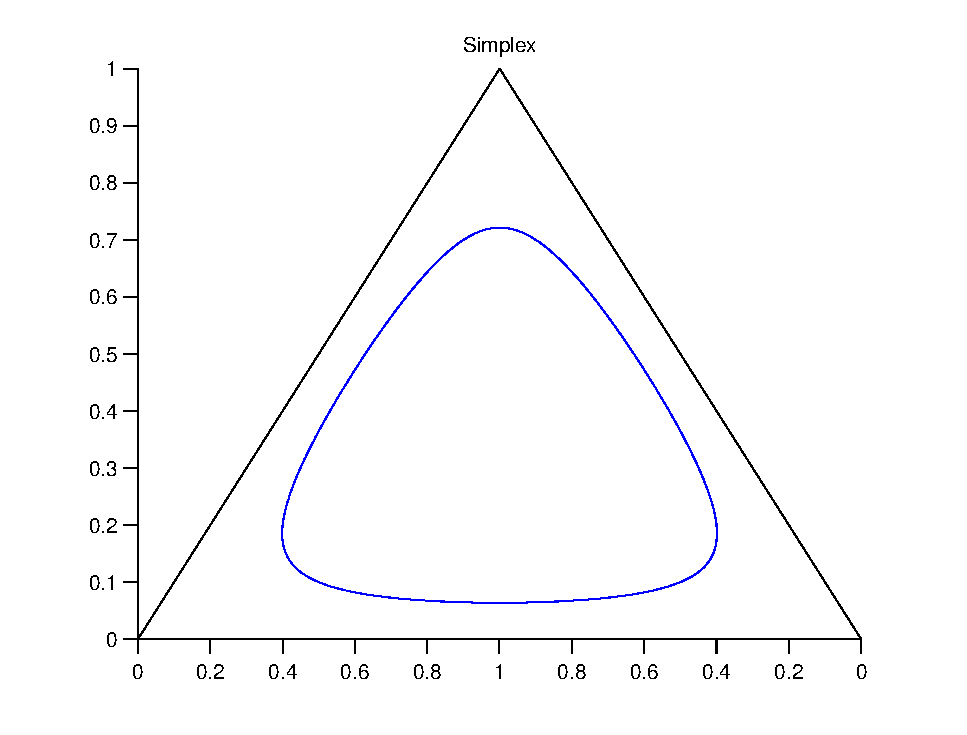
\includegraphics[width=\textwidth]{./images/test1_simplex_rd.eps}
	  \caption{Simplex.}
	  \label{fig:test1_simplex_rd}
  \end{subfigure}
  ~ 
  \begin{subfigure}[b]{0.45\textwidth}
	  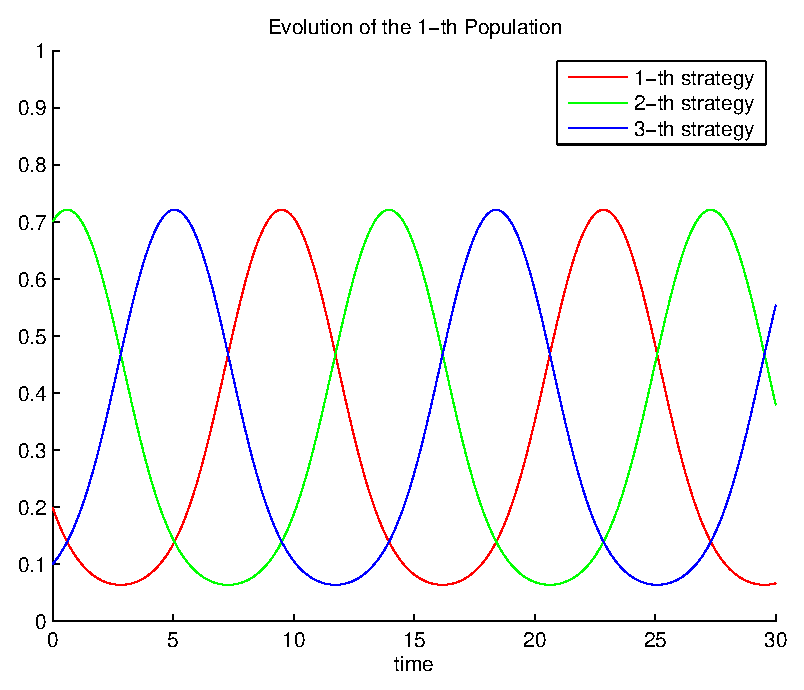
\includegraphics[width=\textwidth]{./images/test1_ev_rd.eps}
	  \caption{Evolution of the strategies in time.}
	  \label{fig:test1_ev_rd}
  \end{subfigure}
  \caption{Rock-paper-scissors game with replicator dynamics.}
  \label{fig:rpc_game_rd}
\end{figure}


\begin{figure}
  \centering
  \begin{subfigure}[b]{0.45\textwidth}
	  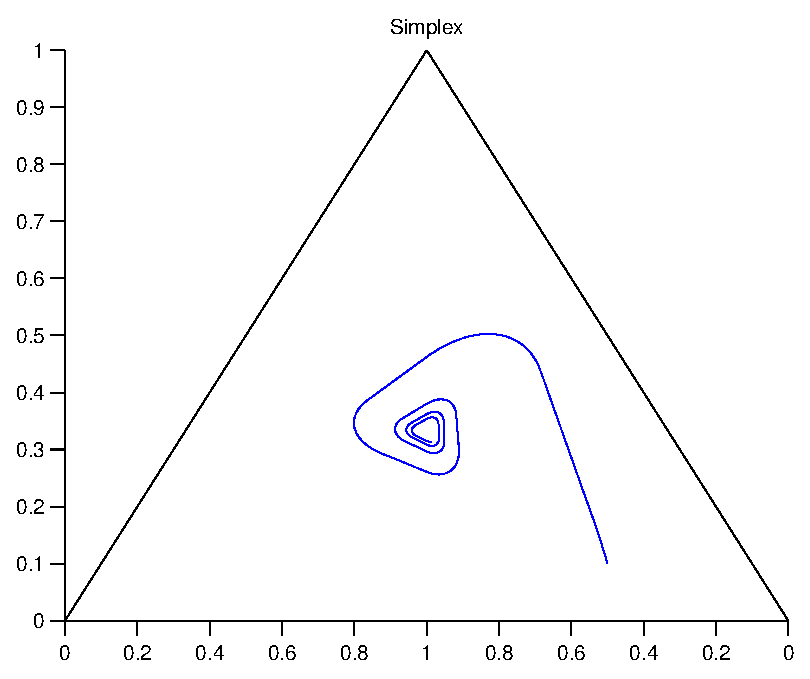
\includegraphics[width=\textwidth]{./images/test1_simplex_bnn.eps}
	  \caption{Simplex.}
	  \label{fig:test1_simplex_bnn}
  \end{subfigure}
  ~ 
  \begin{subfigure}[b]{0.45\textwidth}
	  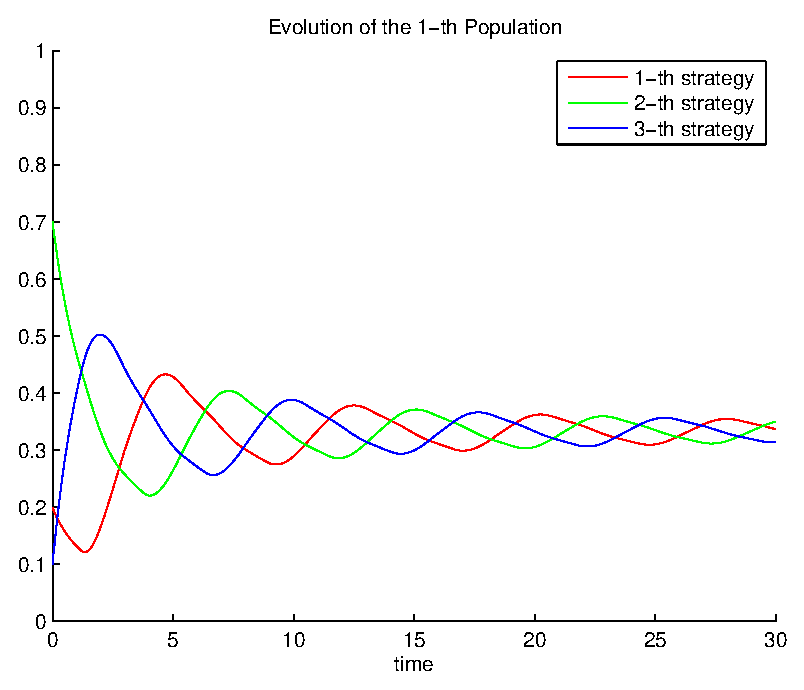
\includegraphics[width=\textwidth]{./images/test1_ev_bnn.eps}
	  \caption{Evolution of the strategies in time.}
	  \label{fig:test1_ev_bnn}
  \end{subfigure}
  \caption{Rock-paper-scissors game with BNN dynamics.}
  \label{fig:rpc_game_bnn}
\end{figure}



\begin{figure}
  \centering
  \begin{subfigure}[b]{0.45\textwidth}
	  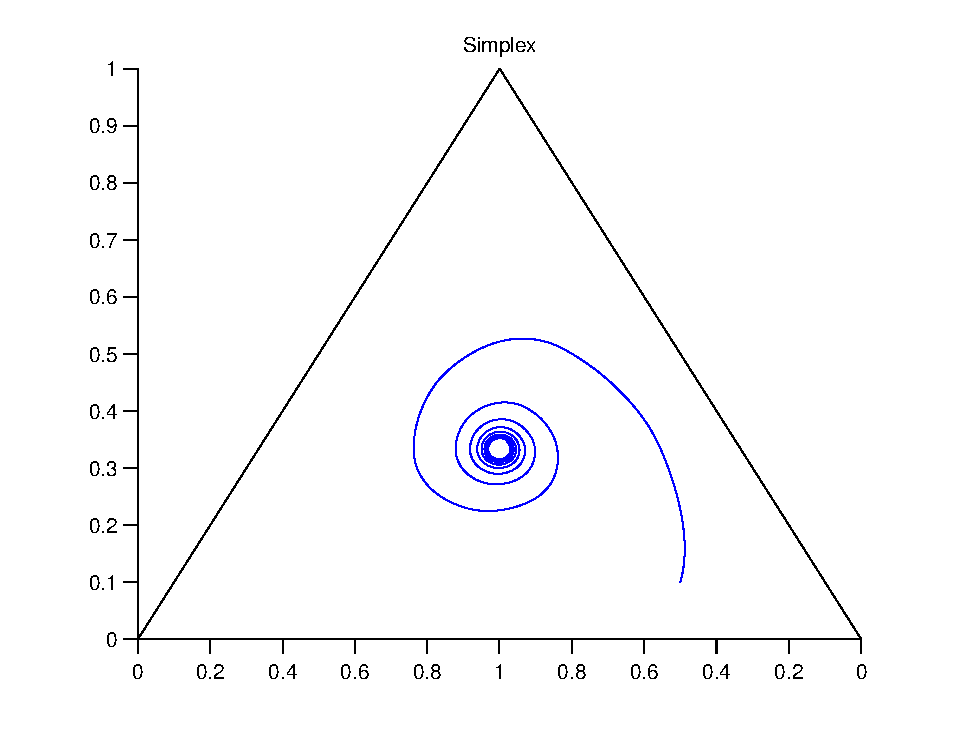
\includegraphics[width=\textwidth]{./images/test1_simplex_smith.eps}
	  \caption{Simplex.}
	  \label{fig:test1_simplex_smith}
  \end{subfigure}
  ~ 
  \begin{subfigure}[b]{0.45\textwidth}
	  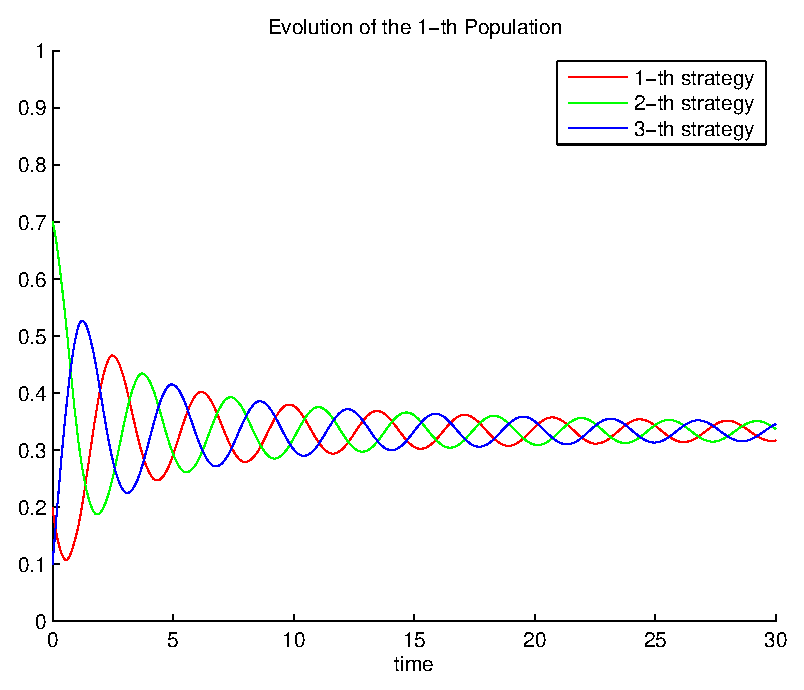
\includegraphics[width=\textwidth]{./images/test1_ev_smith.eps}
	  \caption{Evolution of the strategies in time.}
	  \label{fig:test1_ev_smith}
  \end{subfigure}
  \caption{Rock-paper-scissors game with Smith dynamics.}
  \label{fig:rpc_game_smith}
\end{figure}



\begin{figure}
  \centering
  \begin{subfigure}[b]{0.45\textwidth}
	  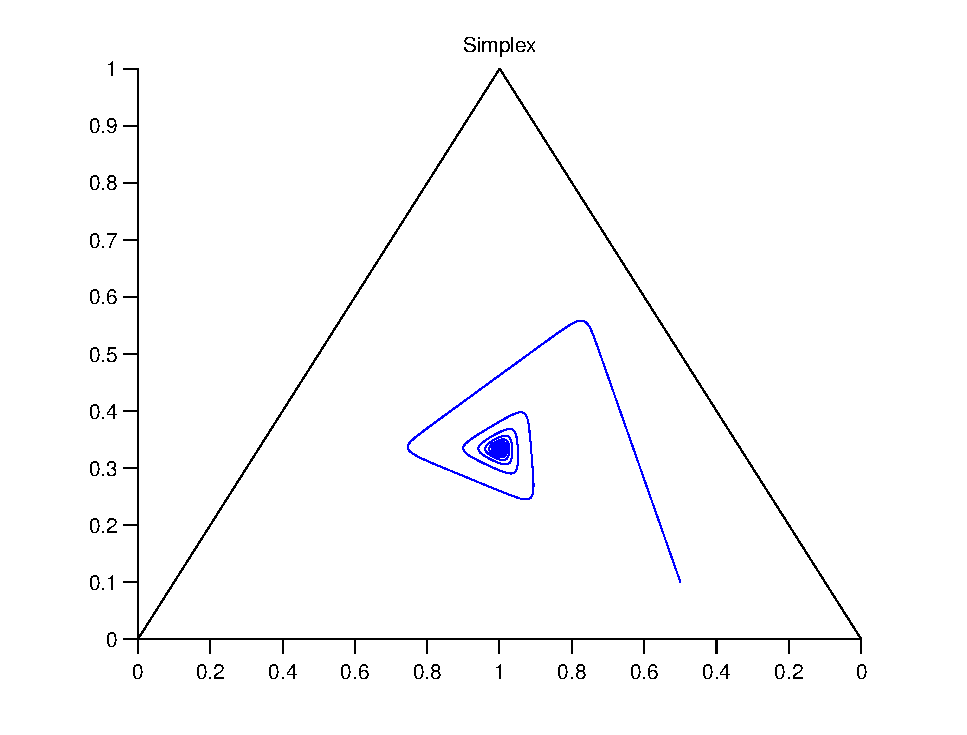
\includegraphics[width=\textwidth]{./images/test1_simplex_logit.eps}
	  \caption{Simplex.}
	  \label{fig:test1_simplex_logit}
  \end{subfigure}
  ~ 
  \begin{subfigure}[b]{0.45\textwidth}
	  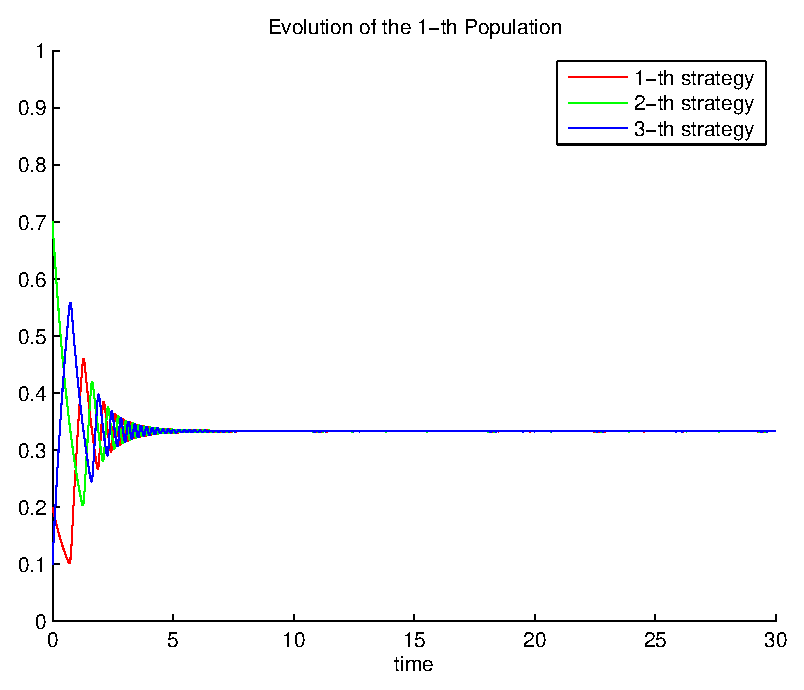
\includegraphics[width=\textwidth]{./images/test1_ev_logit.eps}
	  \caption{Evolution of the strategies in time.}
	  \label{fig:test1_ev_logit}
  \end{subfigure}
  \caption{Rock-paper-scissors game with logit dynamics.}
  \label{fig:rpc_game_logit}
\end{figure}

\fi

